\chapter{Experiment}
\section{Single Joint Examples}\label{sec:simpleExamples}
This section contains step by step examples of how my system functions properly with the hubo system allowing for multiple processes to work with the system

	\subsection{Joint Space Step Response}\label{sec:singlejointStep}
		This section shows the experimental and expected results of controlling a single joint via the Hubo-Ach system.
In this example the right shoulder pitch (RSP) is given a step input from 0.0 $rad$ to 0.4 $rad$.
The reference position $\theta_r$ is begin recorded as well as the actuator setpoint $\theta_c$ and the actual position of the joint $\theta_a$.
These definitions are also available in Table~\ref{table:recorded}

\begin{table}
\centering
\caption{States being recorded for the single joint step response test}
\begin{tabular}{l || c | c | c | c}
Signal      & Symbol     & Definition                    & Source      & Units \\
\hline
\hline
FeedForward & $\theta_r$ & Desired reference on the      & Hubo-Ach   & $rad$ \\
            &            & Hubo-Ach FeedForward Channel  &            &       \\
\hline
FeedForward & $\theta_c$ & Reference set to the actuator & Hubo-Ach   & $rad$ \\
\hline
Feedback    & $\theta_a$ & Actual position of joint as   & JMC        & $rad$ \\
            &            & measured from the encoders    &            &       \\
\hline
\end{tabular}
\label{table:recorded}
\end{table}



\begin{figure}[thpb]
  \centering
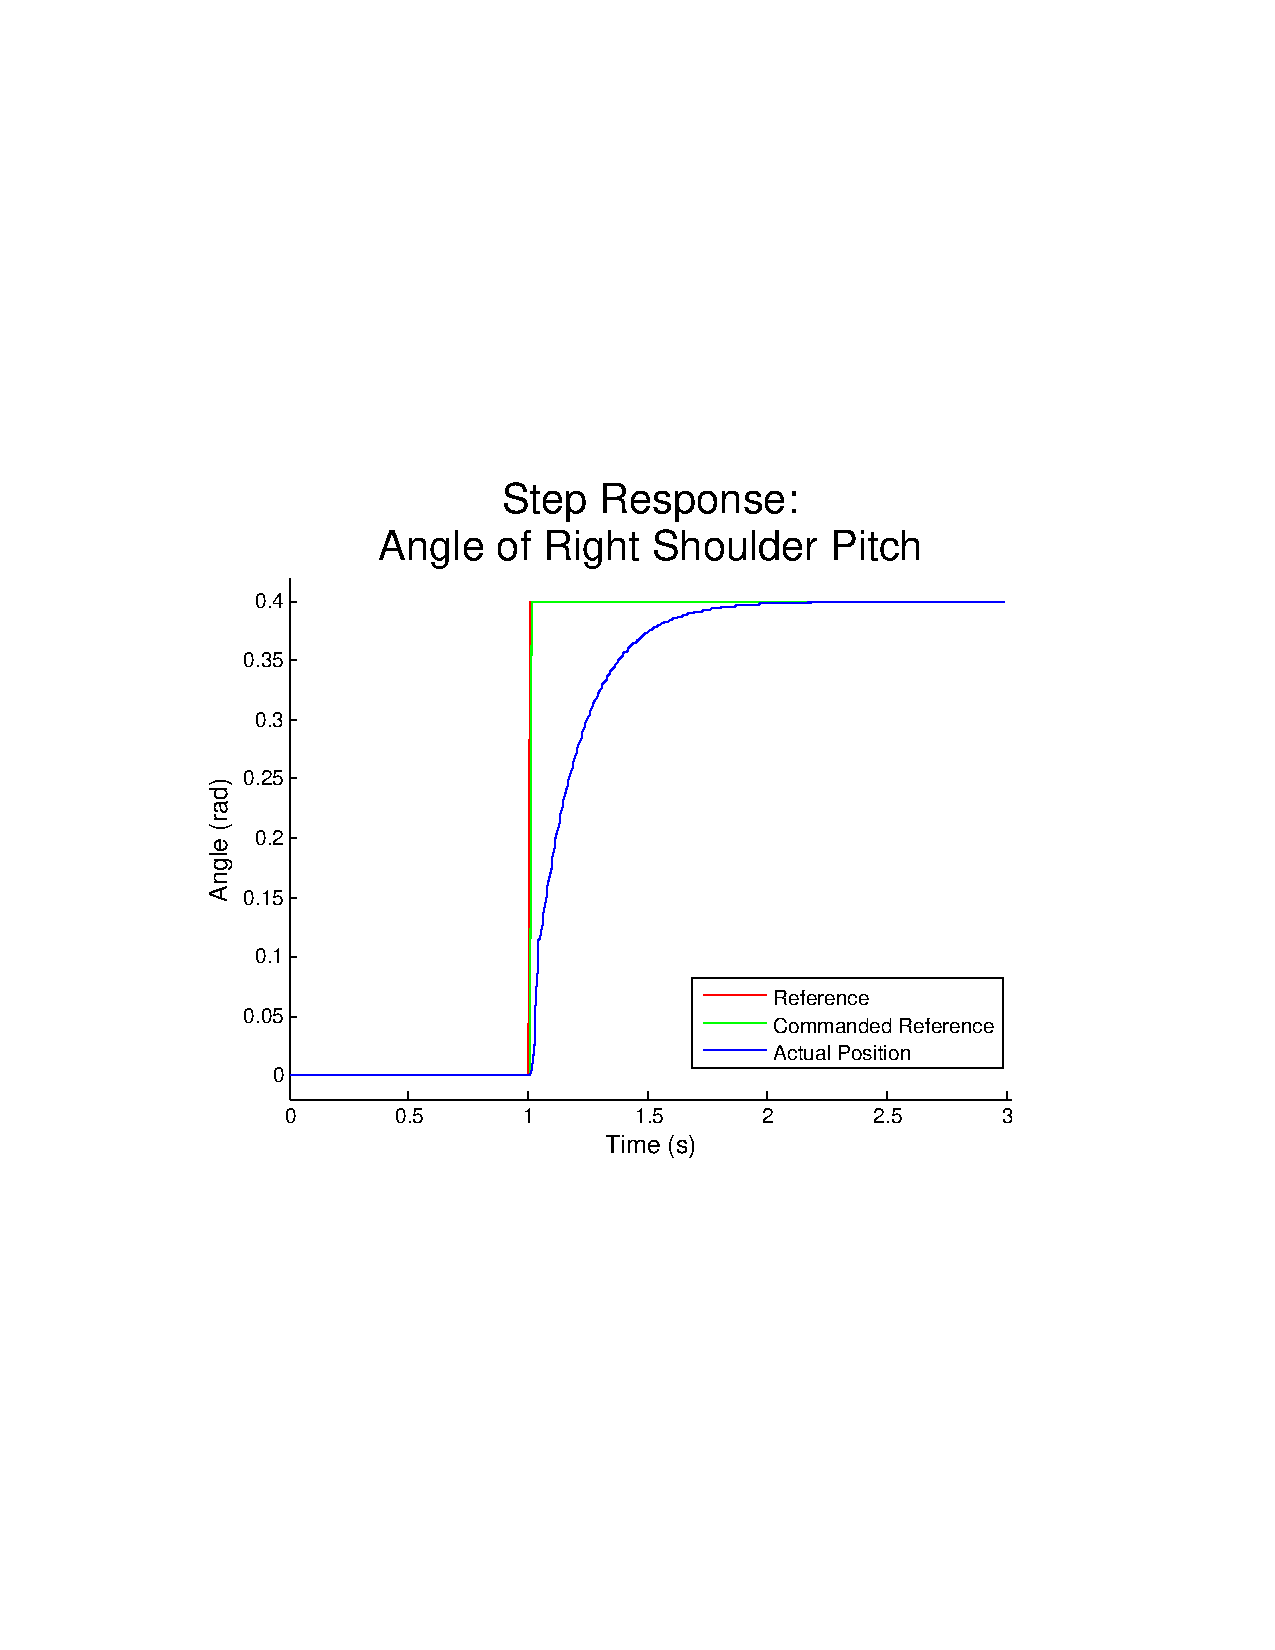
\includegraphics[width=0.8\columnwidth]{./examples/pix/RSP-Zp4-step-step-crop.pdf}
  \caption{The commanded reference plotted against the actual reference recorded via Hubo-Ach and ground truth via CAN analyzing utilities.  In this plot the commanded reference is not automatically filtered by Hubo-Ach.  The commanded joint is the right shoulder pitch.}
  \label{fig:singleJointStep}
\end{figure}

Fig.~\ref{fig:singleJointStep} shows the results when a step input is applied and Hubo-Ach is in \textit{HUBO\_REF\_MODE\_REF\_FILTER} also know as pass-through mode.
This sets the what the desired reference on the \textbf{FeedForward} Hubo-Ach channel to the actuator's reference, i.e.:

\begin{equation}\label{eq:refrefmode}
 \theta_c(N) = \theta_r(N)
\end{equation}

Fig.~\ref{fig:hubo-ach-feedforward} shows the block diagram of the control setup.

\begin{figure}
\centering
\begin{tikzpicture}[->,>=stealth',shorten >=1pt,auto,node distance=5cm,
  thick,main node/.style={fill=white!20,draw,font=\sffamily\Large\bfseries}]


  \node[main node] (ref) {Reference};
  \node[main node] (hubo-ach) [right of=ref] {Hubo-Ach};
  \node[main node] (hubo) [right of=hubo-ach] {Hubo};




  \path[<->,dashed, every node/.style={font=\sffamily\small}]
    (hubo) edge node [above] {CAN} (hubo-ach);

  \path[->,every node/.style={font=\sffamily\small}]
    (ref) edge node [above] {$\theta_r$} (hubo-ach);


\end{tikzpicture}
\caption{Reference $\theta_r$ being applied to Hubo via Hubo-Ach.  $\theta_r$ is set on the \textbf{FeedForward} channel, Hubo-Ach reads it then commands Hubo at the rising edge of the next cycle.}
\label{fig:hubo-ach-feedforward}
\end{figure}






As seen in Fig~\ref{fig:singleJointStep} $\theta_c$ tracks $\theta_r$ perfectly. As expected $\theta_a$ lags by a minimum of 1 time step $T$.  
This is the time it takes between sending $\theta_c$ to the actuator over the CAN bus plus the time it takes in receiving the feedback from the encoder of the motor over CAN.
The remainder of the lag is due to the rise time of the actuator.
This is different for each joint.
Because all major joints are high-gain PID the rise-time and overshoot is very small which makes the robot very stiff.
The total lag between commanding the joint on the \textbf{FeedForward} channel and the response of the actuator is:

\begin{equation}
t_{lag} = t_{filter} + t_{rise}
\end{equation}



	\subsection{Joint Space Step Response with Position Filtering}\label{sec:singlejointFilter}
		Giving a step input to a high-gain PID position controlled actuator can cause an over current fault, burn out motor drivers, strip gears due to the \textit{jerk} etc.  
To reduce this effect Hubo-Ach has multiple modes of on-board filtering.
These modes are:
\begin{itemize}
\item Reference Input Filtering
\item Compliance Amplification 
\end{itemize}

This section talks about \textit{reference input filtering} as a method to apply a step input each joint in joint space and limit the jerk.
It is important to note that the obvious answer is to reduce the PID gains to make the robot \textit{more complaint} however the goal of this work is to make a fully functional system that does not require modification of the robot.
In this case the PID gains are set by the motor drivers and that is considered to be a part of the robot.
In future firmware updates of the motor drivers we will have the ability to change PID gains on the fly.

\textit{reference input filtering} uses the history of the previous $\theta_c$ sent to the given actuator.  The current commanded actuator position $\theta_c(N)$ is given by:

\begin{equation}\label{eq:reffiltermode}
\theta_c(N) = \frac{\theta_c(N-1)\cdot\left(L-1\right) + \theta_r(N)}{L}
\end{equation}

Where $L$ is an integer that represents the length of the filter and $L\geq1$.  
If $L=1$ then Equation~\ref{eq:reffiltermode} becomes Equation~\ref{eq:refrefmode}.



Fig.~\ref{fig:singleJointStepFiltered} shows the commanded reference plotted again the actual reference using the filtered mode defined in Equation~\ref{eq:reffiltermode}.
Fig.~\ref{fig:singleJointStepFilteredLtest} shows the $\theta_r$ plotted against $\theta_c$ and $\theta_a$ for different values of $L$.
It is easy to see that as $L$ increases the $t_{rise}$ also increases and the \textit{jerk} is reduced.


\begin{figure}[thpb]
  \centering
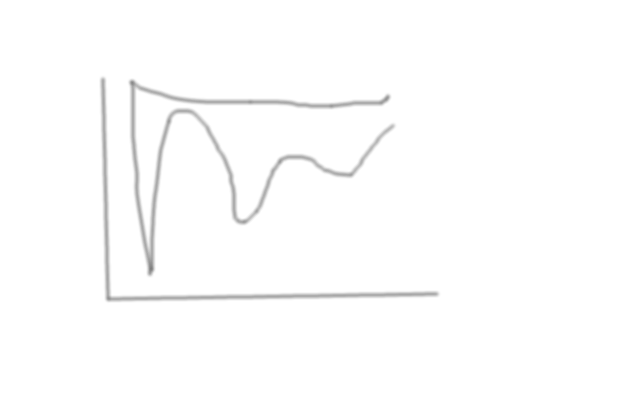
\includegraphics[width=0.8\columnwidth]{./pix/tmp.png}
  \caption{The commanded reference plotted against the actual reference recorded via Hubo-Ach and ground truth via CAN analyzing utilities.  In this plot the commanded reference is automatically filtered by Hubo-Ach.}
  \label{fig:singleJointStepFiltered}
\end{figure}

\begin{figure}[thpb]
  \centering
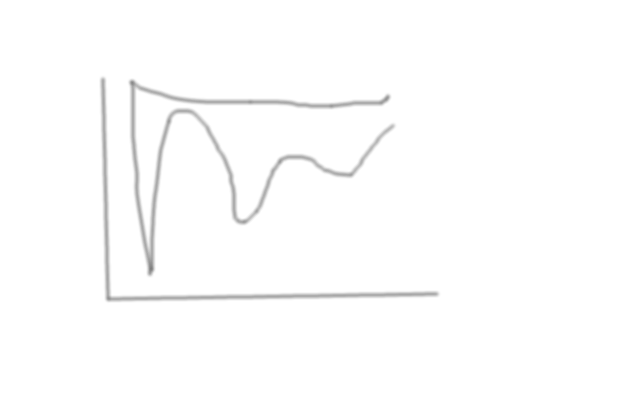
\includegraphics[width=0.8\columnwidth]{./pix/tmp.png}
  \caption{$\theta_r$ plotted against $\theta_c$ and $\theta_a$ recorded via Hubo-Ach with values for $L$ ranging from 1 to 200.}
  \label{fig:singleJointStepFilteredLtest}
\end{figure}

This method is a feed-forward method that assumes that the position you set the actuator to is the actual position of the actuator.

	\subsection{Compliance Amplification}\label{sec:singlejointRefComplience}
		Compliance amplification takes advandage of the internal compliance of the joints and amplifies that by feeding back the PID error $\theta_e$.
Like the Equation~\ref{eq:refrefmode} we have no past information about the set reference and we have only the compiliance given by the joints.
If we think about $\theta_e$ and what effects it we can use it to add compliance to our system.
It is important to note that because the Hubo is a high-gain PID position controlled device with an intergral gain $K_i$ set to zero the steady state error of the joint (the PID error $\theta_e$) is proportional to the moment applied to the joint.
If we combine the reference $\theta_r$ and $\theta_e$ multiplied by a compliance gain $K_c$ we are able to add/amplify the compliance to the system.

\begin{equation}
\theta_c(N) = K_c\theta_e(N)+\theta_r(N)
\end{equation}

It is important to note that $K_c \leq 1$ or the system will go unstable.
If $K_c=1$ then we have

\begin{equation}
\theta_c(N) = \theta_a(N)
\end{equation}

	\subsection{Joint Space Step Response with Feedback Filtering}\label{sec:singlejointEnc}
		Feedback filtering allows us to removes the requirement that we know the joint's current position.
Similar to Equation~\ref{eq:reffiltermode} this method sets $\theta_c$ based on a filter length $L$ and the current desired value $\theta_r$.
However instead of assuming that we know all past $\theta_r$ we use the actual position $\theta_a$.
This method add compliance in a similar way to that of Section~\ref{sec:singlejointRefComplience}.


\begin{equation}\label{eq:refencmode}
\theta_c(N) = \frac{\theta_a(N)\cdot\left(L-1\right) + \theta_r(N)}{L}
\end{equation}

This causes three major effects: 

\noindent \textbf{Effect 1:} The movement of the joint is guaranteed to be filtered even if the previous reference is unknown.

\noindent \textbf{Effect 2:} The steady state error of the feedback filtering method $\theta_e^{fbfilter}$ is greater than that of the PID error $\theta_e$ in the direction of the moment acting on the joint.

\begin{equation}
\theta_e^{fbfilter} > \theta_e
\end{equation}

\noindent \textbf{Effect 3:} The joint's compliance has increased due to the effect of the moment applied to the joint has on the steady state error.

\begin{figure}
\centering

\begin{tikzpicture}[->,>=stealth',shorten >=1pt,auto,node distance=5cm,
  thick,main node/.style={fill=white!20,draw,font=\sffamily\Large\bfseries}]


  \node[main node] (ref) {Reference};
  \node[main node] (filter) [right=3.0cm of ref] {Filter};
  \node[main node] (hubo-ach) [below=1.0cm of filter] {Hubo-Ach};
  \node[main node] (hubo) [right=3.0cm of hubo-ach] {Hubo};




  \path[<->,dashed, every node/.style={font=\sffamily\small}]
    (hubo) edge node [above] {CAN} (hubo-ach);

  \path[->,every node/.style={font=\sffamily\small}]
    (ref) edge node [above] {$\theta_d$} (filter);

  \path[->,every node/.style={font=\sffamily\small}]
    (hubo-ach) edge node [left] {$\theta_r$} (filter);

  \path[->,every node/.style={font=\sffamily\small}]
    (filter) edge node [right] {$\theta_a$} (hubo-ach);


% look into this and add z^-1

\path [every node/.style={draw,minimum width=3cm, minimum height=5cm]}]
  node (a) at (0,0) {}
  [xshift=7cm]
  node (b) at (0,0) {}
  [xshift=7cm]
  node (c) at (0,0) {};

%\begin{scope}[->,>=latex]
%    \foreach \i in {-2,...,2}{% 
%      \draw[->] ([yshift=\i * 0.8 cm]a.east) -- ([yshift=\i * 0.8 cm]b.west) ;}

%    \foreach \i in {1,2}{% 
%      \draw[->] ([yshift=\i * 0.8 cm]a.east) to [out=50,in=130] ([yshift=\i * 0.8 cm]c.west) ;} 

%    \foreach \i in {-1,-2}{% 
%      \draw[->] ([yshift=\i * 0.8 cm]a.east) to [out=-50,in=-130] ([yshift=\i * 0.8 cm]c.west) ;}
%\end{scope}


\end{tikzpicture}
\caption{Desired reference $\theta_d$ being filtered before applied to Hubo via Hubo-Ach.  $\theta_d$ is sent through a filter that reduces the \textit{jerk} on the actuator then the new reference $\theta_r$ is set on the \textbf{FeedForward} channel, Hubo-Ach reads it then commands Hubo at the rising edge of the next cycle.}
\label{fig:hubo-ach-feedforward}
\end{figure}



Fig.~\ref{fig:singleJointStepFilteredFeedback} shows $\theta_r$ plotted against $\theta_c$ and $\theta_a$.  
$\theta_a$ not only lags behind $\theta_c$ but it also has a greater steady state error.
Fig.~\ref{fig:singleJointStepFilteredFeedbackMoment} shows how the steady state error $\theta_e^{fbfilter}$ increases with an applied moment.
This is where we get our compliance.

\begin{figure}[thpb]
  \centering
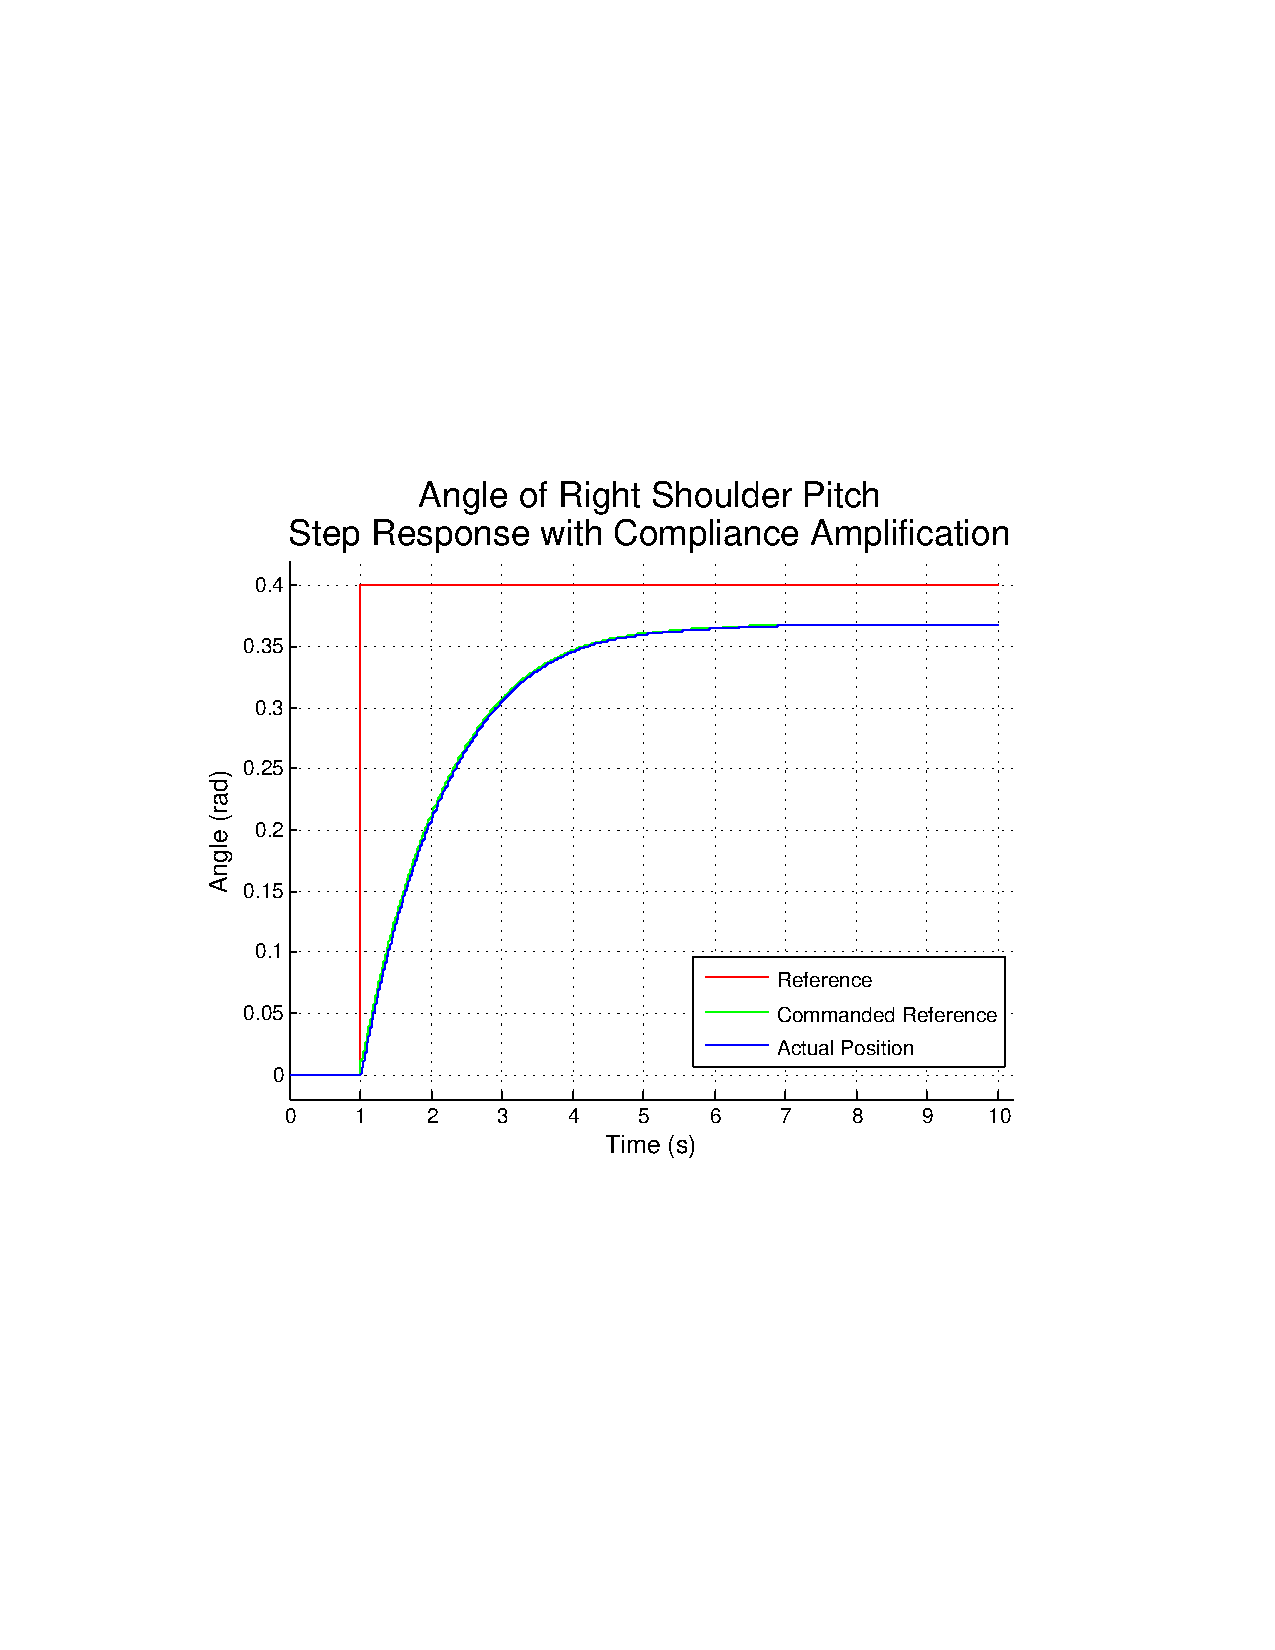
\includegraphics[width=0.8\columnwidth]{./examples/pix/RSP-Zp4-step-enc-real-crop.pdf}
  \caption{$\theta_r$ plotted against $\theta_c$ and $\theta_a$ recorded via Hubo-Ach using the feedback filtering method.}
  \label{fig:singleJointStepFilteredFeedback}
\end{figure}

\begin{figure}[thpb]
  \centering
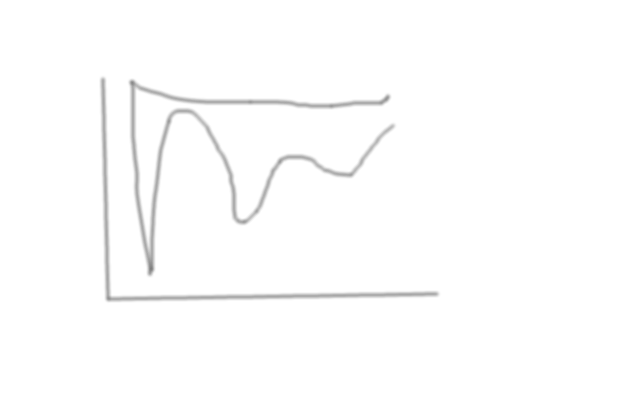
\includegraphics[width=0.8\columnwidth]{./pix/tmp.png}
  \caption{$\theta_r$ plotted against $\theta_c$ and $\theta_a$ recorded via Hubo-Ach using the feedback filtering method with different moments applied to the joint.  You will note that as the moment increases so does $\theta_e^{fbfilter}$. }
  \label{fig:singleJointStepFilteredFeedbackMoment}
\end{figure}

\section{Six Degree of Freedom Inverse Kinimatic Implimentation Example}\label{sec:6dofik}
This section shows how we calculate the inverse kinimatics (IK) for the Hubo's right arm and how we use that calculation in conjunction with Section~\ref{sec:simpleExamples}.  The result is the ability to command the end effector (EEF)
%	\subsection{Work Space Controller Example}
%		The next step is to find the inverse kinematic (IK) solution for the right arm.
Inherently this problem has multiple solutions.
When solving the IK Pieper\cite{peiper1968kinematics} states that a closed-form solution does exist if:
\begin{itemize}
\item Three consecutive joints axes of the manipulator are parallel to one another
\end{itemize}

OR
\begin{itemize}
\item Three consecutive joints intercect at a single point
\end{itemize}

The kinematic structure in Fig~\ref{fig:hubo} and Fig~\ref{fig:IkFkCoordinate} shows that the Hubo2+ platform does have a three joints that intersect the same point in the shoulders and in the hips.
Thus a closed-form solution exists for both arms and both legs.

The transform $T_0^6$ in Equation~\ref{eq:t06} is needed to solve the IK problem for the shoulder.  
It is important to note that $T_0^6$ is in the form of

\begin{equation}\label{eq:T06}
T_0^6 = \left[ \begin{array}{cccc} 
\overline{x_6} & \overline{y_6} & \overline{z_6} & \overline{p_6} \\
0              & 0              & 0              & 1   
\end{array} \right]
\end{equation} 

Where $\overline{x_6}$, $\overline{y_6}$ and $\overline{z_6}$ are $[3x1]$ unit vectors along the principle axes of the end-effectors coordinate frame $i$, see Fig.~\ref{fig:IkFkCoordinate}.
Position vector $\overline{p_6}$ describes the hand about joint $A1$ (shoulder).
The arm can be vied in different frames.
If we look at the arm in reference to the end-effector's frame.
The reverse transform is defined as $(T_0^6)`$


\begin{equation}
(T_0^6)' = T_6^0 = (T_0^6)^{-1} = \left[ \begin{array}{cccc} 
\overline{x_6} & \overline{y_6} & \overline{z_6} & \overline{p_6} \\
0              & 0              & 0              & 1   
\end{array} \right]^{-1}
\end{equation} 

The following method is based on the work done by our partner Park et. al.\cite{5649842}.
The general link translation matrix $T_{i-1}^i$ relates the $i^{th}$ coordinate frame to the $(i-1)^{th}$ coordinate frame.  
In addition we can extend Equation~\ref{eq:T06} to

\begin{equation}\label{eq:06invIK}
T_0^6 = \left[ \begin{array}{cccc} 
\overline{x_6} & \overline{y_6} & \overline{z_6} & \overline{p_6} \\
0              & 0              & 0              & 1   
\end{array} \right] = \left[ \begin{array}{cccc} 
\overline{n} & \overline{s} & \overline{a} & \overline{p} \\
0            & 0            & 0            & 1   
\end{array} \right]
\end{equation} 

Where $[\overline{n}, \overline{s}, \overline{a}, \overline{p}]$ represents the normal vector, the sliding vector, the approach vector and the position vector of the end effector respectively\cite{fu1987robotics}.  We can now state that

\begin{equation}
(T_0^6)' = T_6^0 = (T_0^6)^{-1} = \left[ \begin{array}{cccc} 
\overline{x_6} & \overline{y_6} & \overline{z_6} & \overline{p_6} \\
0              & 0              & 0              & 1   
\end{array} \right]^{-1}= \left[ \begin{array}{cccc} 
\overline{n}' & \overline{s}' & \overline{a}' & \overline{p}' \\
0             & 0             & 0             & 1   
\end{array} \right]
\end{equation} 

We can now use the reverse method to solve for the joint angles as in \cite{fu1987robotics} and derived in the tech report\cite{gtechIK2}.
The first three lower joint angles of $A_4$, $A_5$ and $A_6$ are solved for.
Subsequently the upper joint angles of $A_1$, $A_2$ and $A_3$ are solved.

Using inverse transform methods\cite{4046335} we can modify Equation~\ref{eq:t06} to

\begin{equation}\label{eq:t06IK}
T_6^0 = (T_0^6)^{-1} = \prod_{i=6}^{1} T_{i}^{i-1} = T_{6}^{5}T_{5}^{4}T_{4}^{3}T_{3}^{2}T_{2}^{1}T_{1}^{0}
\end{equation}

Then we equate Equation~\ref{eq:06invIK} to Equation~\ref{eq:t06IK} 

\begin{equation}
T_{6}^{5}T_{5}^{4}T_{4}^{3}T_{3}^{2}T_{2}^{1}T_{1}^{0} = \left[ \begin{array}{cccc} 
\overline{n}' & \overline{s}' & \overline{a}' & \overline{p}' \\
0             & 0             & 0             & 1   
\end{array} \right]
\end{equation}

Then move $T_6^5$ to the other side of the equation


\begin{equation}\label{eq:preG}
T_{5}^{4}T_{4}^{3}T_{3}^{2}T_{2}^{1}T_{1}^{0} = T_{5}^{6}\left[ \begin{array}{cccc} 
\overline{n}' & \overline{s}' & \overline{a}' & \overline{p}' \\
0             & 0             & 0             & 1   
\end{array} \right]
\end{equation}

For simplicity we will represent Equation~\ref{eq:preG} as $G_L$ and $G_R$ standing for \textit{right} and \textit{left} side.

\begin{equation}
G_L = T_{5}^{6}\left[ \begin{array}{cccc} 
\overline{n}' & \overline{s}' & \overline{a}' & \overline{p}' \\
0             & 0             & 0             & 1   
\end{array} \right]
\end{equation}



\begin{equation}
G_R = T_{5}^{4}T_{4}^{3}T_{3}^{2}T_{2}^{1}T_{1}^{0} 
\end{equation}


Expanding gives us

\begin{equation}
G_L = \left[ \begin{array}{cccc} 
g_{11} & g_{12} & g_{13} & cos(\theta_6)(p_x'+l_{A_4})-sin(\theta_6)p_y' \\
g_{21} & g_{22} & g_{23} & sin(\theta_6)(p_x'+l_{A_4})-cos(\theta_6)p_y' \\
g_{31} & g_{32} & g_{33} & p_z'                                         \\
0      & 0      & 0      & 1   
\end{array} \right]
\end{equation}

and

\begin{equation}
G_R = \left[ \begin{array}{cccc} 
g_{11} & g_{12} & g_{13} & sin(\theta_4)cos(\theta_5)l_{A_2} \\
g_{21} & g_{22} & g_{23} & -cos(\theta_6)l_{A_2}-l_{A3}       \\
g_{31} & g_{32} & g_{33} & sin(\theta_4)sin(\theta_5)l_{A_2}  \\
0      & 0      & 0      & 1   
\end{array} \right]
\end{equation}

We can then equate elements $(1,4)$, $(2,4)$ and $(3,4)$ of $G_L$ and $G_R$. 
This gives us

\begin{equation}\label{eq:thetaSolve11}
cos(\theta_6)(p_x'+l_{A_4})-sin(\theta_6)p_y' = sin(\theta_4)cos(\theta_5)l_{A_2}
\end{equation}

\begin{equation}\label{eq:thetaSolve12}
sin(\theta_6)(p_x'+l_{A_4})-cos(\theta_6)p_y' = -cos(\theta_6)l_{A_2}-l_{A3}
\end{equation}

\begin{equation}\label{eq:thetaSolve13}
p_z' = sin(\theta_4)sin(\theta_5)l_{A_2}
\end{equation}

Based on the desired task space location we let

\begin{equation}\label{eq:thetaSolve21}
p_x' + l_{A_4} = r \cdot cos(\phi)
\end{equation}

and

\begin{equation}\label{eq:thetaSolve22}
p_y' = r \cdot sin(\phi)
\end{equation}

where 

\begin{equation}\label{eq:thetaSolve31}
r = sqrt{(p_x'+l_{A_4})^2 + (p_y')^2}
\end{equation}

and 

\begin{equation}\label{eq:thetaSolve32}
\phi = atan2(p_y',p_x'+l_{A_4})
\end{equation}

\textbf{Note:} $atan2()$ represents the the $atan$ method that gathers the information of the signs of the inputs in order to put the returned value in the appropriate quadrant.

Combining Equation (\ref{eq:thetaSolve11}), (\ref{eq:thetaSolve12}) and (\ref{eq:thetaSolve13}) with Equation (\ref{eq:thetaSolve21}) and (\ref{eq:thetaSolve22}) we get

\begin{equation}\label{eq:thetaSolve41}
r \cdot cos(\theta_6+\phi) = sin(\theta_4)cos(\theta_5)l_{A_2}
\end{equation}

\begin{equation}\label{eq:thetaSolve42}
r \cdot sin(\theta_6+\phi) = -cos(\theta_4)l_{A_2}-l_{A_3}
\end{equation}

\begin{equation}\label{eq:thetaSolve43}
p_z' = sin(\theta_4)sin(\theta_5)l_{A_2}
\end{equation}


When we combine above with Equation (\ref{eq:thetaSolve31}) and (\ref{eq:thetaSolve32}) and obtain 


\begin{equation}
\theta_4 = atan2\left( \pm \sqrt{1-cos(\theta_4)^2} , cos(\theta_4)  \right)
\end{equation}

where

\begin{equation}
cos(\theta_4) = \frac{(p_x'+l_{A_4})^2  +  p_y'^2  +  p_z'^2  -  l_{A_2}^2  -  l_{A_3}^2}
                     {2l_{A_2}l_{A3}}
\end{equation}

Using Equation~\ref{eq:thetaSolve43} we can get $\theta_5$

\begin{equation}
\theta_5 = atan2(sin(\theta_5), \pm\sqrt{1-sin(\theta_5)^2})
\end{equation}

where

\begin{equation}
sin(\theta_5) = \frac{p_z'}
                     {sin(\theta_4)l_{A_2}}
\end{equation}


We can then solve for $\theta_6$ by dividing Equation~\ref{eq:thetaSolve42} by Equation~\ref{eq:thetaSolve41}.



\begin{equation}
\frac{r \cdot sin(\theta_6+\phi)}
     {r \cdot cos(\theta_6+\phi)} = tan(\theta_6+\phi) = \frac{-cos(\theta_4)l_{A_2}-l_{A_3}}
                                                              {sin(\theta_4)cos(\theta_5)l_{A_2}}
\end{equation}

\begin{equation}
\theta_6 = atan2(-(cos(\theta_4)l_{A_2}+l_{A_3}), sin(\theta_4)cos(\theta_5)l_{A_2}) - \phi
\end{equation}


%	\subsection{Six DOF IK Implimentaiton}
In order to control the Hubo's upper body manipulators in work space as opposed to joint space both forward and inverse kinematics are required, (FK) and (IK) respectively.
In order to find a proper solution the joint limits, singularities and feasible workspace (no-self collisions) must be accounted for.

The kinematic structure of the right and left arm of the Hubo are identical with the caveat that the work space offset is mirrored over the z-axis.
This means that they have the same Denavit–Hartenberg (DH) parameters.

\begin{table}
\centering
\caption{Denavit–Hartenberg for Hubo2+ upper body (arms) in standard format}
\begin{tabular}{|l | c|}
\hline
Link     & Length (m) \\
\hline
\hline
$l_{A1}$ & 0.215 \\
\hline
$l_{A2}$ & 0.179 \\
\hline
$l_{A3}$ & 0.182 \\
\hline
$l_{A4}$ & 0.121 \\
\hline
$l_{E}$ & 0.100 \\

\hline

\end{tabular}\label{table:DHupper}
\end{table}

\begin{figure}
\centering

\begin{tikzpicture}[->,>=stealth',shorten >=1pt,auto,node distance=5cm,
  thick,main node/.style={fill=white!20,draw,font=\sffamily\small\bfseries}]

  \node[main node] (ref) [text width=3cm] {End Effector Position};

  \node[main node] (ik) [right=2.0cm of ref] {6-DOF IK};
  \node[main node] (filter) [right=2.0cm of ik] {Filter};
  \node[main node] (hubo-ach) [below=1.0cm of filter] {Hubo-Ach};
  \node[main node] (hubo) [right=2.0cm of hubo-ach] {Hubo};



  \path[->, every node/.style={font=\sffamily\small}]
    (ref) edge node [above] {$(x,y,z)$} (ik)
    (ref) edge node [below] {$(\alpha,\beta,\gamma)$} (ik);
%  \path[->, every node/.style={font=\sffamily\small}]
%    (ref) edge node [below] {$(\alpha,\beta,\gamma)$} (ik);

 

  \path[->,every node/.style={font=\sffamily\small}]
    (ik) edge node [above] {$\overline{\theta_d}$} (filter);

 \draw[->] ([xshift=-0.5 cm]filter.south)  -- node [left] {$\overline{\theta_r}$} ([xshift=-0.5 cm]hubo-ach.north)  ;
 \draw[->] ([xshift=0.5 cm]hubo-ach.north) -- node [left] {$\overline{\theta_a}$} ([xshift=0.5 cm]filter.south)  ;

 \path[<->,dashed, every node/.style={font=\sffamily\small}]
    (hubo) edge node [above] {CAN} (hubo-ach);

%  \path[->,every node/.style={font=\sffamily\small}]
%    (hubo-ach) edge node [left] {$\theta_r$} (filter);

%  \path[->,every node/.style={font=\sffamily\small}]
%    (filter) edge node [right] {$\theta_a$} (hubo-ach);




% look into this and add z^-1

%\path [every node/.style={draw,minimum width=3cm, minimum height=5cm]}]
%  node (a) at (0,0) {}
%  [xshift=7cm]
%  node (b) at (0,0) {}
%  [xshift=7cm]
%  node (c) at (0,0) {};

%\begin{scope}[->,>=latex]
%    \foreach \i in {-2,...,2}{% 
%      \draw[->] ([yshift=\i * 0.8 cm]a.east) -- ([yshift=\i * 0.8 cm]b.west) ;}

%    \foreach \i in {1,2}{% 
%      \draw[->] ([yshift=\i * 0.8 cm]a.east) to [out=50,in=130] ([yshift=\i * 0.8 cm]c.west) ;} 

%    \foreach \i in {-1,-2}{% 
%      \draw[->] ([yshift=\i * 0.8 cm]a.east) to [out=-50,in=-130] ([yshift=\i * 0.8 cm]c.west) ;}
%\end{scope}


\end{tikzpicture}
\caption{Desired reference $\theta_d$ being filtered before applied to Hubo via Hubo-Ach.  $\theta_d$ is sent through a filter that reduces the \textit{jerk} on the actuator by using Equation~\ref{eq:refencmode}.  The new reference $\theta_r$ is set on the \textbf{FeedForward} channel, Hubo-Ach reads it then commands Hubo at the rising edge of the next cycle.  This method adds compliance to the system}
\label{fig:hubo-ach-feedforwardFilterFeedBack}
\end{figure}



	\subsection{Froward Kinematics} 
		The transform between joint adjacent joints is represented by the transform:

\begin{equation}
T_i^{i-1} = \left[ \begin{array}{cccc} 
cos(\theta_i) & -sin(\theta_i)cos(\alpha_i) &  sin(\theta_i)sin(\alpha_i)  &  a_i cos(\theta_i) \\ 
sin(\theta_i) &  cos(\theta_i)cos(\alpha_i) & -cos(\theta_i)sin(\alpha_i)  &  a_i sin(\theta_i) \\
0             &  sin(\alpha_i)              &  cos(\alpha_i)               &  d_i               \\
0             &  0                          &  0                           &  1                 
\end{array} \right]
\end{equation}

Where $\theta_i$ is the 

\begin{figure}[thpb]
  \centering
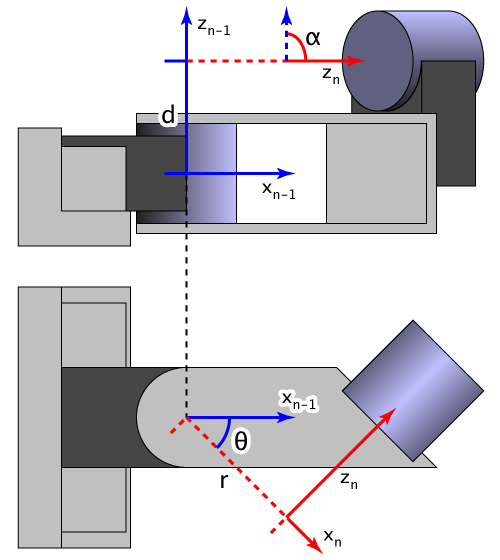
\includegraphics[width=0.8\columnwidth]{./examples/pix/Sample_Denavit-Hartenberg_Diagram.png}

	\subsection{Inverse Kinematics}
			The next step is to find the inverse kinematic (IK) solution for the right arm.
Inherently this problem has multiple solutions.
When solving the IK Pieper\cite{peiper1968kinematics} states that a closed-form solution does exist if:
\begin{itemize}
\item Three consecutive joints axes of the manipulator are parallel to one another
\end{itemize}

OR
\begin{itemize}
\item Three consecutive joints intercect at a single point
\end{itemize}

The kinematic structure in Fig~\ref{fig:hubo} and Fig~\ref{fig:IkFkCoordinate} shows that the Hubo2+ platform does have a three joints that intersect the same point in the shoulders and in the hips.
Thus a closed-form solution exists for both arms and both legs.

The transform $T_0^6$ in Equation~\ref{eq:t06} is needed to solve the IK problem for the shoulder.  
It is important to note that $T_0^6$ is in the form of

\begin{equation}\label{eq:T06}
T_0^6 = \left[ \begin{array}{cccc} 
\overline{x_6} & \overline{y_6} & \overline{z_6} & \overline{p_6} \\
0              & 0              & 0              & 1   
\end{array} \right]
\end{equation} 

Where $\overline{x_6}$, $\overline{y_6}$ and $\overline{z_6}$ are $[3x1]$ unit vectors along the principle axes of the end-effectors coordinate frame $i$, see Fig.~\ref{fig:IkFkCoordinate}.
Position vector $\overline{p_6}$ describes the hand about joint $A1$ (shoulder).
The arm can be vied in different frames.
If we look at the arm in reference to the end-effector's frame.
The reverse transform is defined as $(T_0^6)`$


\begin{equation}
(T_0^6)' = T_6^0 = (T_0^6)^{-1} = \left[ \begin{array}{cccc} 
\overline{x_6} & \overline{y_6} & \overline{z_6} & \overline{p_6} \\
0              & 0              & 0              & 1   
\end{array} \right]^{-1}
\end{equation} 

The following method is based on the work done by our partner Park et. al.\cite{5649842}.
The general link translation matrix $T_{i-1}^i$ relates the $i^{th}$ coordinate frame to the $(i-1)^{th}$ coordinate frame.  
In addition we can extend Equation~\ref{eq:T06} to

\begin{equation}\label{eq:06invIK}
T_0^6 = \left[ \begin{array}{cccc} 
\overline{x_6} & \overline{y_6} & \overline{z_6} & \overline{p_6} \\
0              & 0              & 0              & 1   
\end{array} \right] = \left[ \begin{array}{cccc} 
\overline{n} & \overline{s} & \overline{a} & \overline{p} \\
0            & 0            & 0            & 1   
\end{array} \right]
\end{equation} 

Where $[\overline{n}, \overline{s}, \overline{a}, \overline{p}]$ represents the normal vector, the sliding vector, the approach vector and the position vector of the end effector respectively\cite{fu1987robotics}.  We can now state that

\begin{equation}
(T_0^6)' = T_6^0 = (T_0^6)^{-1} = \left[ \begin{array}{cccc} 
\overline{x_6} & \overline{y_6} & \overline{z_6} & \overline{p_6} \\
0              & 0              & 0              & 1   
\end{array} \right]^{-1}= \left[ \begin{array}{cccc} 
\overline{n}' & \overline{s}' & \overline{a}' & \overline{p}' \\
0             & 0             & 0             & 1   
\end{array} \right]
\end{equation} 

We can now use the reverse method to solve for the joint angles as in \cite{fu1987robotics} and derived in the tech report\cite{gtechIK2}.
The first three lower joint angles of $A_4$, $A_5$ and $A_6$ are solved for.
Subsequently the upper joint angles of $A_1$, $A_2$ and $A_3$ are solved.

Using inverse transform methods\cite{4046335} we can modify Equation~\ref{eq:t06} to

\begin{equation}\label{eq:t06IK}
T_6^0 = (T_0^6)^{-1} = \prod_{i=6}^{1} T_{i}^{i-1} = T_{6}^{5}T_{5}^{4}T_{4}^{3}T_{3}^{2}T_{2}^{1}T_{1}^{0}
\end{equation}

Then we equate Equation~\ref{eq:06invIK} to Equation~\ref{eq:t06IK} 

\begin{equation}
T_{6}^{5}T_{5}^{4}T_{4}^{3}T_{3}^{2}T_{2}^{1}T_{1}^{0} = \left[ \begin{array}{cccc} 
\overline{n}' & \overline{s}' & \overline{a}' & \overline{p}' \\
0             & 0             & 0             & 1   
\end{array} \right]
\end{equation}

Then move $T_6^5$ to the other side of the equation


\begin{equation}\label{eq:preG}
T_{5}^{4}T_{4}^{3}T_{3}^{2}T_{2}^{1}T_{1}^{0} = T_{5}^{6}\left[ \begin{array}{cccc} 
\overline{n}' & \overline{s}' & \overline{a}' & \overline{p}' \\
0             & 0             & 0             & 1   
\end{array} \right]
\end{equation}

For simplicity we will represent Equation~\ref{eq:preG} as $G_L$ and $G_R$ standing for \textit{right} and \textit{left} side.

\begin{equation}
G_L = T_{5}^{6}\left[ \begin{array}{cccc} 
\overline{n}' & \overline{s}' & \overline{a}' & \overline{p}' \\
0             & 0             & 0             & 1   
\end{array} \right]
\end{equation}



\begin{equation}
G_R = T_{5}^{4}T_{4}^{3}T_{3}^{2}T_{2}^{1}T_{1}^{0} 
\end{equation}


Expanding gives us

\begin{equation}
G_L = \left[ \begin{array}{cccc} 
g_{11} & g_{12} & g_{13} & cos(\theta_6)(p_x'+l_{A_4})-sin(\theta_6)p_y' \\
g_{21} & g_{22} & g_{23} & sin(\theta_6)(p_x'+l_{A_4})-cos(\theta_6)p_y' \\
g_{31} & g_{32} & g_{33} & p_z'                                         \\
0      & 0      & 0      & 1   
\end{array} \right]
\end{equation}

and

\begin{equation}
G_R = \left[ \begin{array}{cccc} 
g_{11} & g_{12} & g_{13} & sin(\theta_4)cos(\theta_5)l_{A_2} \\
g_{21} & g_{22} & g_{23} & -cos(\theta_6)l_{A_2}-l_{A3}       \\
g_{31} & g_{32} & g_{33} & sin(\theta_4)sin(\theta_5)l_{A_2}  \\
0      & 0      & 0      & 1   
\end{array} \right]
\end{equation}

We can then equate elements $(1,4)$, $(2,4)$ and $(3,4)$ of $G_L$ and $G_R$. 
This gives us

\begin{equation}\label{eq:thetaSolve11}
cos(\theta_6)(p_x'+l_{A_4})-sin(\theta_6)p_y' = sin(\theta_4)cos(\theta_5)l_{A_2}
\end{equation}

\begin{equation}\label{eq:thetaSolve12}
sin(\theta_6)(p_x'+l_{A_4})-cos(\theta_6)p_y' = -cos(\theta_6)l_{A_2}-l_{A3}
\end{equation}

\begin{equation}\label{eq:thetaSolve13}
p_z' = sin(\theta_4)sin(\theta_5)l_{A_2}
\end{equation}

Based on the desired task space location we let

\begin{equation}\label{eq:thetaSolve21}
p_x' + l_{A_4} = r \cdot cos(\phi)
\end{equation}

and

\begin{equation}\label{eq:thetaSolve22}
p_y' = r \cdot sin(\phi)
\end{equation}

where 

\begin{equation}\label{eq:thetaSolve31}
r = sqrt{(p_x'+l_{A_4})^2 + (p_y')^2}
\end{equation}

and 

\begin{equation}\label{eq:thetaSolve32}
\phi = atan2(p_y',p_x'+l_{A_4})
\end{equation}

\textbf{Note:} $atan2()$ represents the the $atan$ method that gathers the information of the signs of the inputs in order to put the returned value in the appropriate quadrant.

Combining Equation (\ref{eq:thetaSolve11}), (\ref{eq:thetaSolve12}) and (\ref{eq:thetaSolve13}) with Equation (\ref{eq:thetaSolve21}) and (\ref{eq:thetaSolve22}) we get

\begin{equation}\label{eq:thetaSolve41}
r \cdot cos(\theta_6+\phi) = sin(\theta_4)cos(\theta_5)l_{A_2}
\end{equation}

\begin{equation}\label{eq:thetaSolve42}
r \cdot sin(\theta_6+\phi) = -cos(\theta_4)l_{A_2}-l_{A_3}
\end{equation}

\begin{equation}\label{eq:thetaSolve43}
p_z' = sin(\theta_4)sin(\theta_5)l_{A_2}
\end{equation}


When we combine above with Equation (\ref{eq:thetaSolve31}) and (\ref{eq:thetaSolve32}) and obtain 


\begin{equation}
\theta_4 = atan2\left( \pm \sqrt{1-cos(\theta_4)^2} , cos(\theta_4)  \right)
\end{equation}

where

\begin{equation}
cos(\theta_4) = \frac{(p_x'+l_{A_4})^2  +  p_y'^2  +  p_z'^2  -  l_{A_2}^2  -  l_{A_3}^2}
                     {2l_{A_2}l_{A3}}
\end{equation}

Using Equation~\ref{eq:thetaSolve43} we can get $\theta_5$

\begin{equation}
\theta_5 = atan2(sin(\theta_5), \pm\sqrt{1-sin(\theta_5)^2})
\end{equation}

where

\begin{equation}
sin(\theta_5) = \frac{p_z'}
                     {sin(\theta_4)l_{A_2}}
\end{equation}


We can then solve for $\theta_6$ by dividing Equation~\ref{eq:thetaSolve42} by Equation~\ref{eq:thetaSolve41}.



\begin{equation}
\frac{r \cdot sin(\theta_6+\phi)}
     {r \cdot cos(\theta_6+\phi)} = tan(\theta_6+\phi) = \frac{-cos(\theta_4)l_{A_2}-l_{A_3}}
                                                              {sin(\theta_4)cos(\theta_5)l_{A_2}}
\end{equation}

\begin{equation}
\theta_6 = atan2(-(cos(\theta_4)l_{A_2}+l_{A_3}), sin(\theta_4)cos(\theta_5)l_{A_2}) - \phi
\end{equation}


			
\section{Visual Serving Example}
This section uses visual feedback using an RGB-D (Red Green Blue - Depth) camera and the 6-DOF IK example from Section~\ref{sec:6dofik}.
	\subsection{Tracking Using Vision}
		Using a simple HSV (Hue Saturation Value) 

		
		
\section{Valve Turning}
	\begin{figure}[thpb]
  \centering
  %\begin{tikzpicture}
    %\clip [rounded corners=1em] (0,0) rectangle coordinate (centerpoint) (5,7.5cm);
%    \node[minimum width=\linewidth,minimum height=174pt,draw=black,rounded corners=1em,fill=bgcolor,draw=black]
%    {};
%    \node[name=img] {
      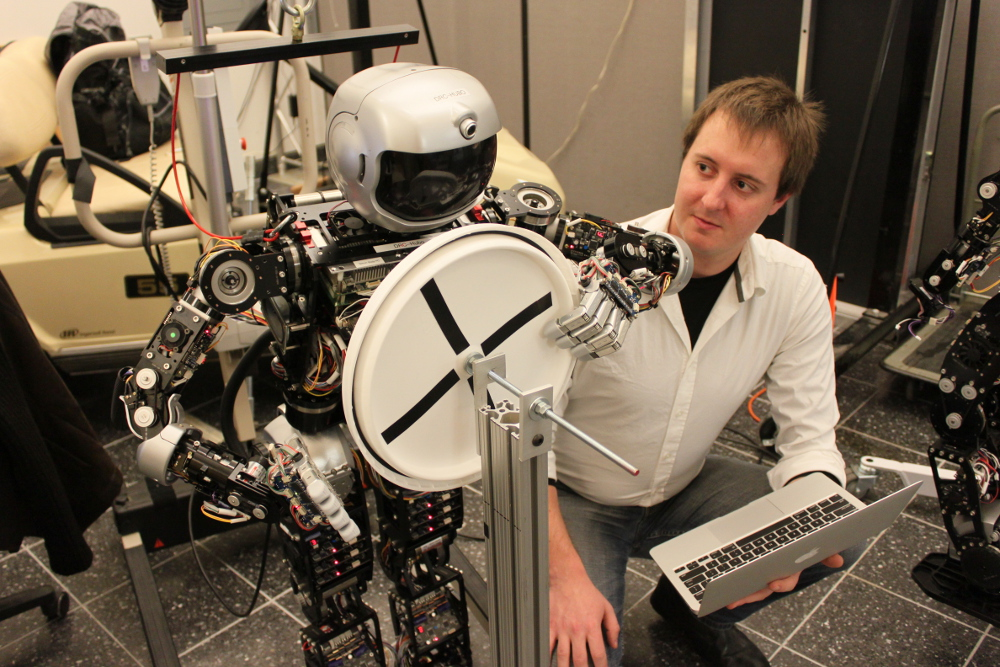
\includegraphics[width=0.93\columnwidth]{./pix/IMG_9107-small.jpg}
      
\includegraphics{./qrcode/qrcode-valve.png}\\
      Video: http://danlofaro.com/phd/valve/
%    };
%    \draw [bgcolor, rounded corners=1em, line width=1em,inner sep=0pt]
%    (img.north west) --
%    (img.north east) --
%    (img.south east) --
%    (img.south west) -- cycle
%    ;
%  \end{tikzpicture}
\caption{Hubo (left) turning a valve via Hubo-Ach alongside Daniel
  M. Lofaro (right).  Valve turning developed in conjunction with
  Dmitry Berenson at WPI for the DARPA Robotics Challenge.}
  \label{fig:valve}
\end{figure}

\section{Walking}
	This section shows examples of how Hubo-Ach was used for stable walking.
Examples are given using:
\begin{itemize}
\item Hubo2+ (Physical Robot)
\item OpenHubo (Simulator)
\item RobotSim Hubo (Simulator)
\end{itemize}

section~\ref{sec:WalkingPatternGeneration} shows how the open-loop walking trajectory is created.

Section~\ref{sec:OpenHuboWalking} shows how the open loop walking trajectory is run in sim-time on OpenHubo using Hubo-Ach.
Section~\ref{sec:RobotSimWalking} shows how the open loop walking trajectory is run in sim-time on RobotSim using Hubo-Ach.
Section~\ref{sec:HuboWalking} shows the same walking trajectory running on the real Hubo hardware in real-time using Hubo-Ach.
It also shows the difference between running in sim-time and real-time.
Section~\ref{sec:dynamicWalking} shows the result of a five day \textit{hack-a-thon} using Hubo-Ach to add dynamic walking capability.





%% ---------------- Walking Pattern Generation ------------------------
\subsection{Walking Pattern Generation}\label{sec:WalkingPatternGeneration}
The walking pattern demonstrated in this section is generated based on the work of Park et. al.\cite{4115633}
A walking pattern is the way in which a legged robot, in this case two legged, moves its joints to create a walking gate while maintaining stability.
The walking pattern consists of two major phases:
\begin{itemize}
\item Single Support Phase (SSP)
\item Double Support Phase (DSP)
\end{itemize}

\noindent \textbf{Single support phase} is when one foot is on the ground.
This phase is when one leg moves from one stepping position to the other.
The ZMP must remain above the planted foot to guarantee stability.\\

\noindent \textbf{Double support phase} is when both feet are planted on the ground.  
When in this phase the ZMP moves from above one foot to the other along the stable area as seen in Fig.~\ref{fig:zmp}.




\begin{figure}[t]
  \centering
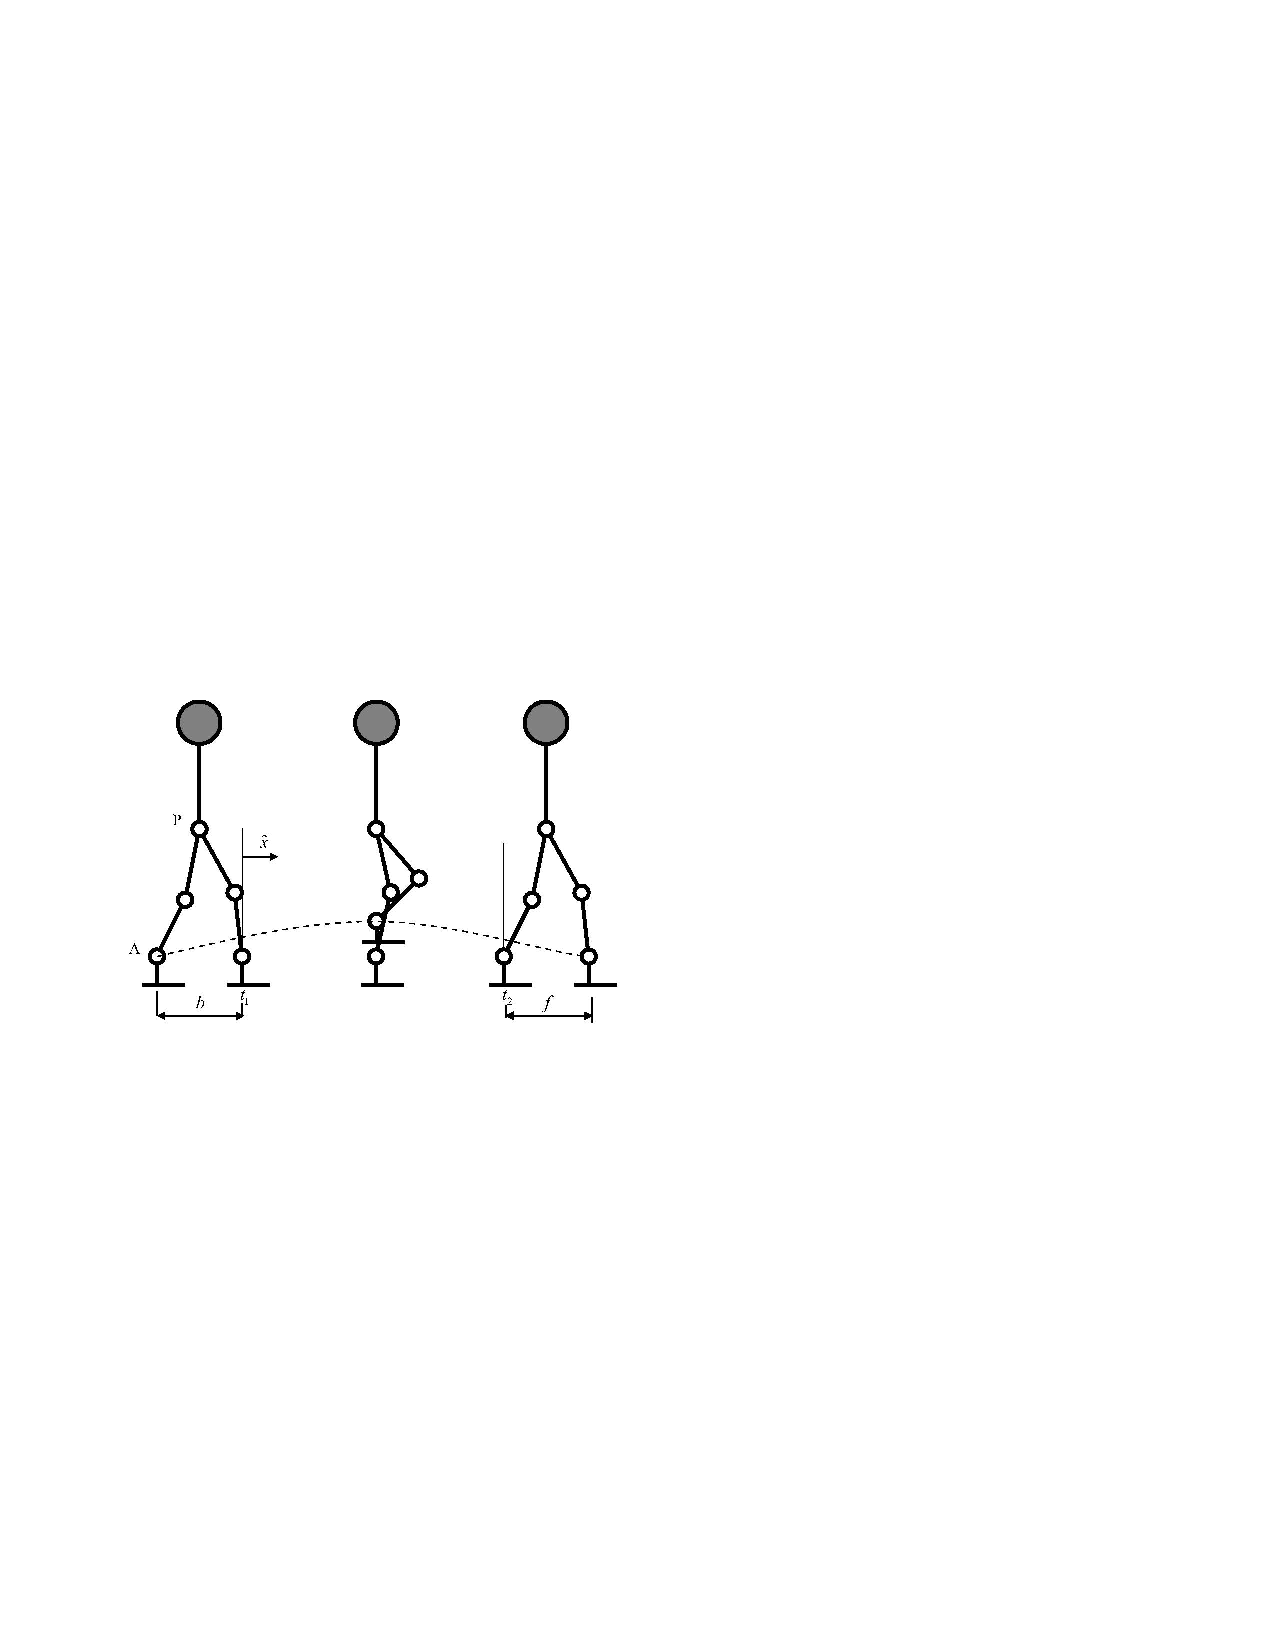
\includegraphics[width=0.5\columnwidth]{./examples/pix/huboZMPx.pdf}
  \caption{Hubo model diagram for ZMP walking in the $x$ direction (side view).  $b$ and $f$ are the step lengths for the left and the right foot.  $A$ defines the ankle.  $t_1$ is the time of the starting of the step, $t_2$ defines the landing of the stepping foot.  $P$ defines the hip location.  $\widetilde{x}$ defines the walking velocity.  The middle diagram depicts the SSP and the left and right diagrams show the DSP.}
  \label{fig:huboZMPx}
\end{figure}

Fig~\ref{fig:huboZMPx} and \ref{fig:huboZMPy} shows the walking pattern phases on a Hubo model in the $x$ and $y$ direction respectively.
In these figures $A_R$ and $A_L$ defines the left and right ankles respectively.  
$t_1$ is the time of the starting of the step, $t_2$ defines the landing of the stepping foot.  
$t_0$ defines time when the stepping foot is at peak step height.  
$P$ defines the hip location.  
$\widetilde{x}$ defines the walking velocity.
$\widetilde{y}$ defines the body sway velocity.  
The middle diagram depicts the SSP and the left and right diagrams show the DSP.



\begin{figure}[t]
  \centering
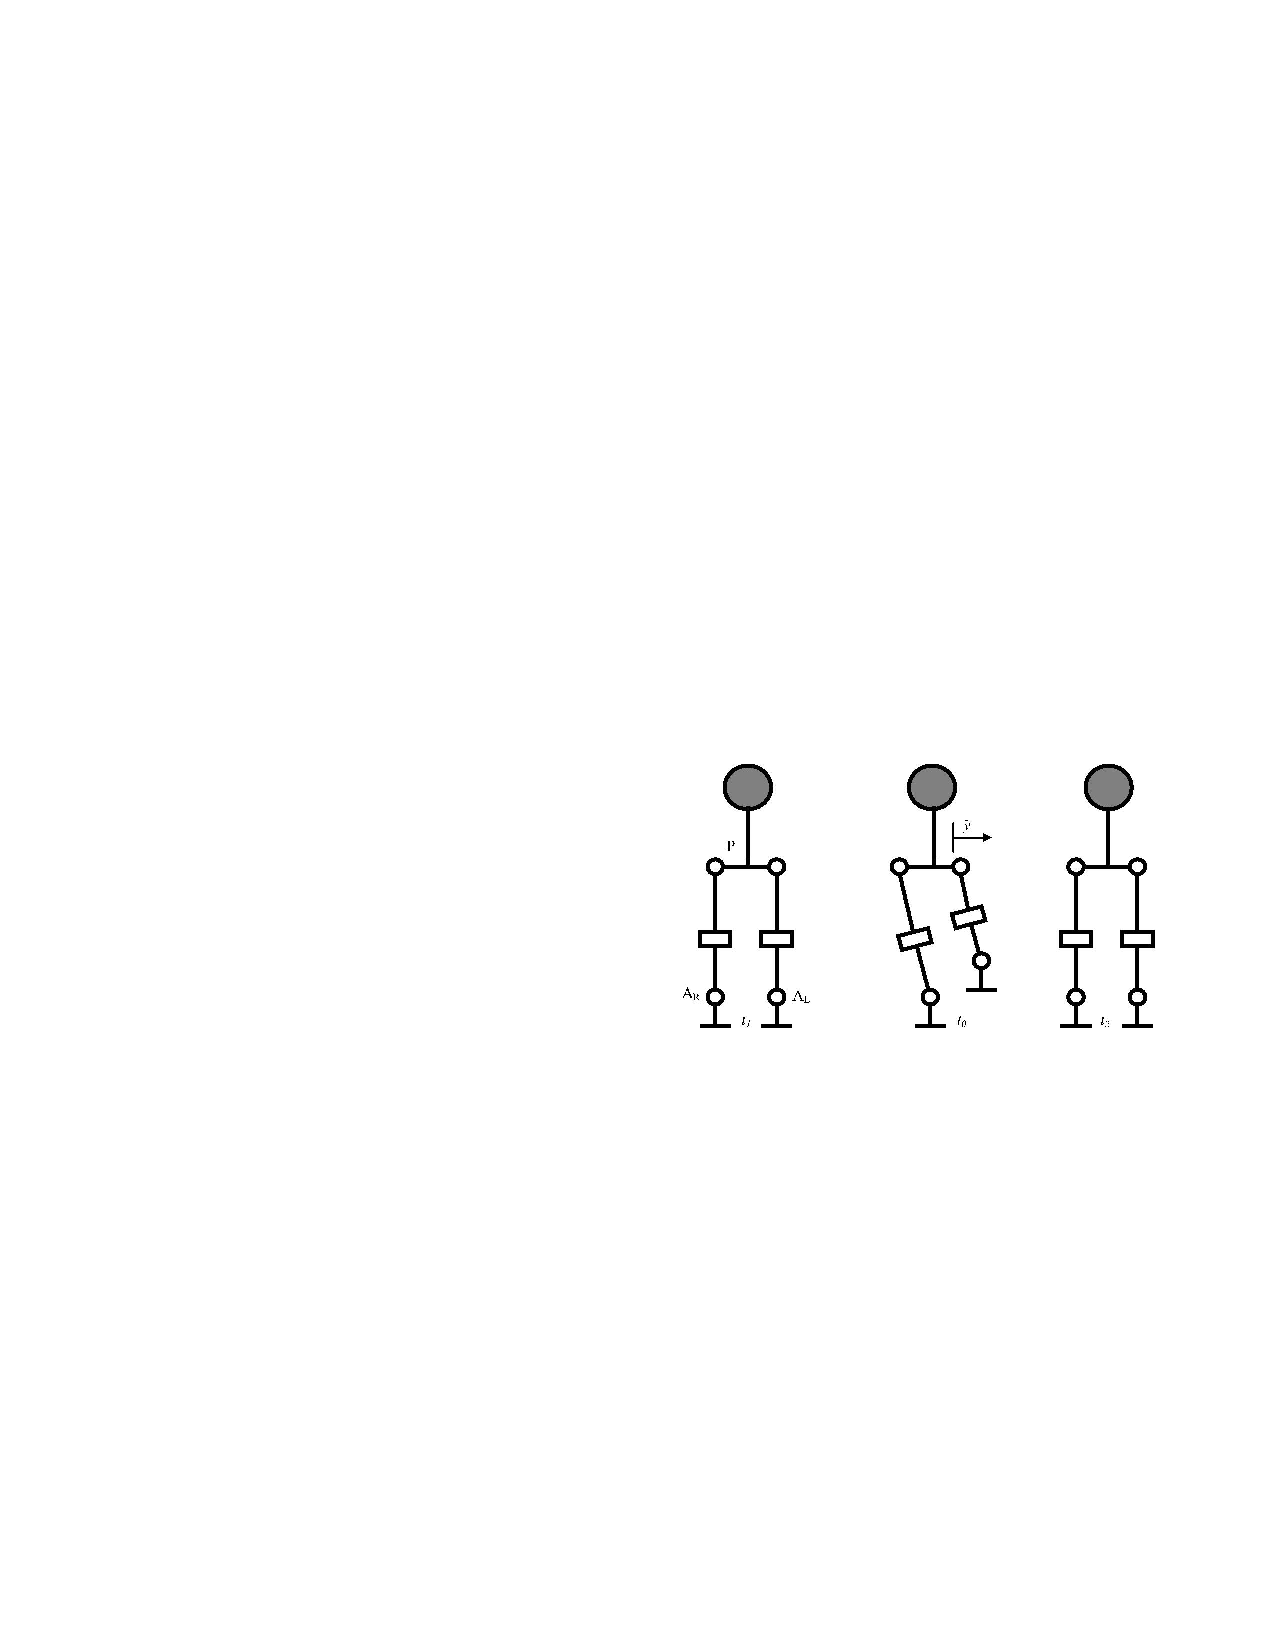
\includegraphics[width=0.7\columnwidth]{./examples/pix/huboZMPy.pdf}
  \caption{Hubo model diagram for ZMP walking in the $y$ direction (front view).  $A_R$ and $A_L$ defines the left and right ankles respectively.  $t_1$ is the time of the starting of the step, $t_2$ defines the landing of the stepping foot.  $t_0$ defines time when the stepping foot is at peak step height.  $P$ defines the hip location.  $\widetilde{y}$ defines the body sway velocity.  The middle diagram depicts the SSP and the left and right diagrams show the DSP.}
  \label{fig:huboZMPy}
\end{figure}


The walking patterns are generated creating a joint space trajectory with a period $T$ of $0.005~sec$.
The patterns keep the ZMP criteria described in Section~\ref{sec:zmp}.
These walking patterns are used to test the simulated robots and the physical robots.
Fig.~\ref{fig:huboZMPjointSpace} shows the joint space walking pattern verses time.

\begin{figure}[t]
  \centering
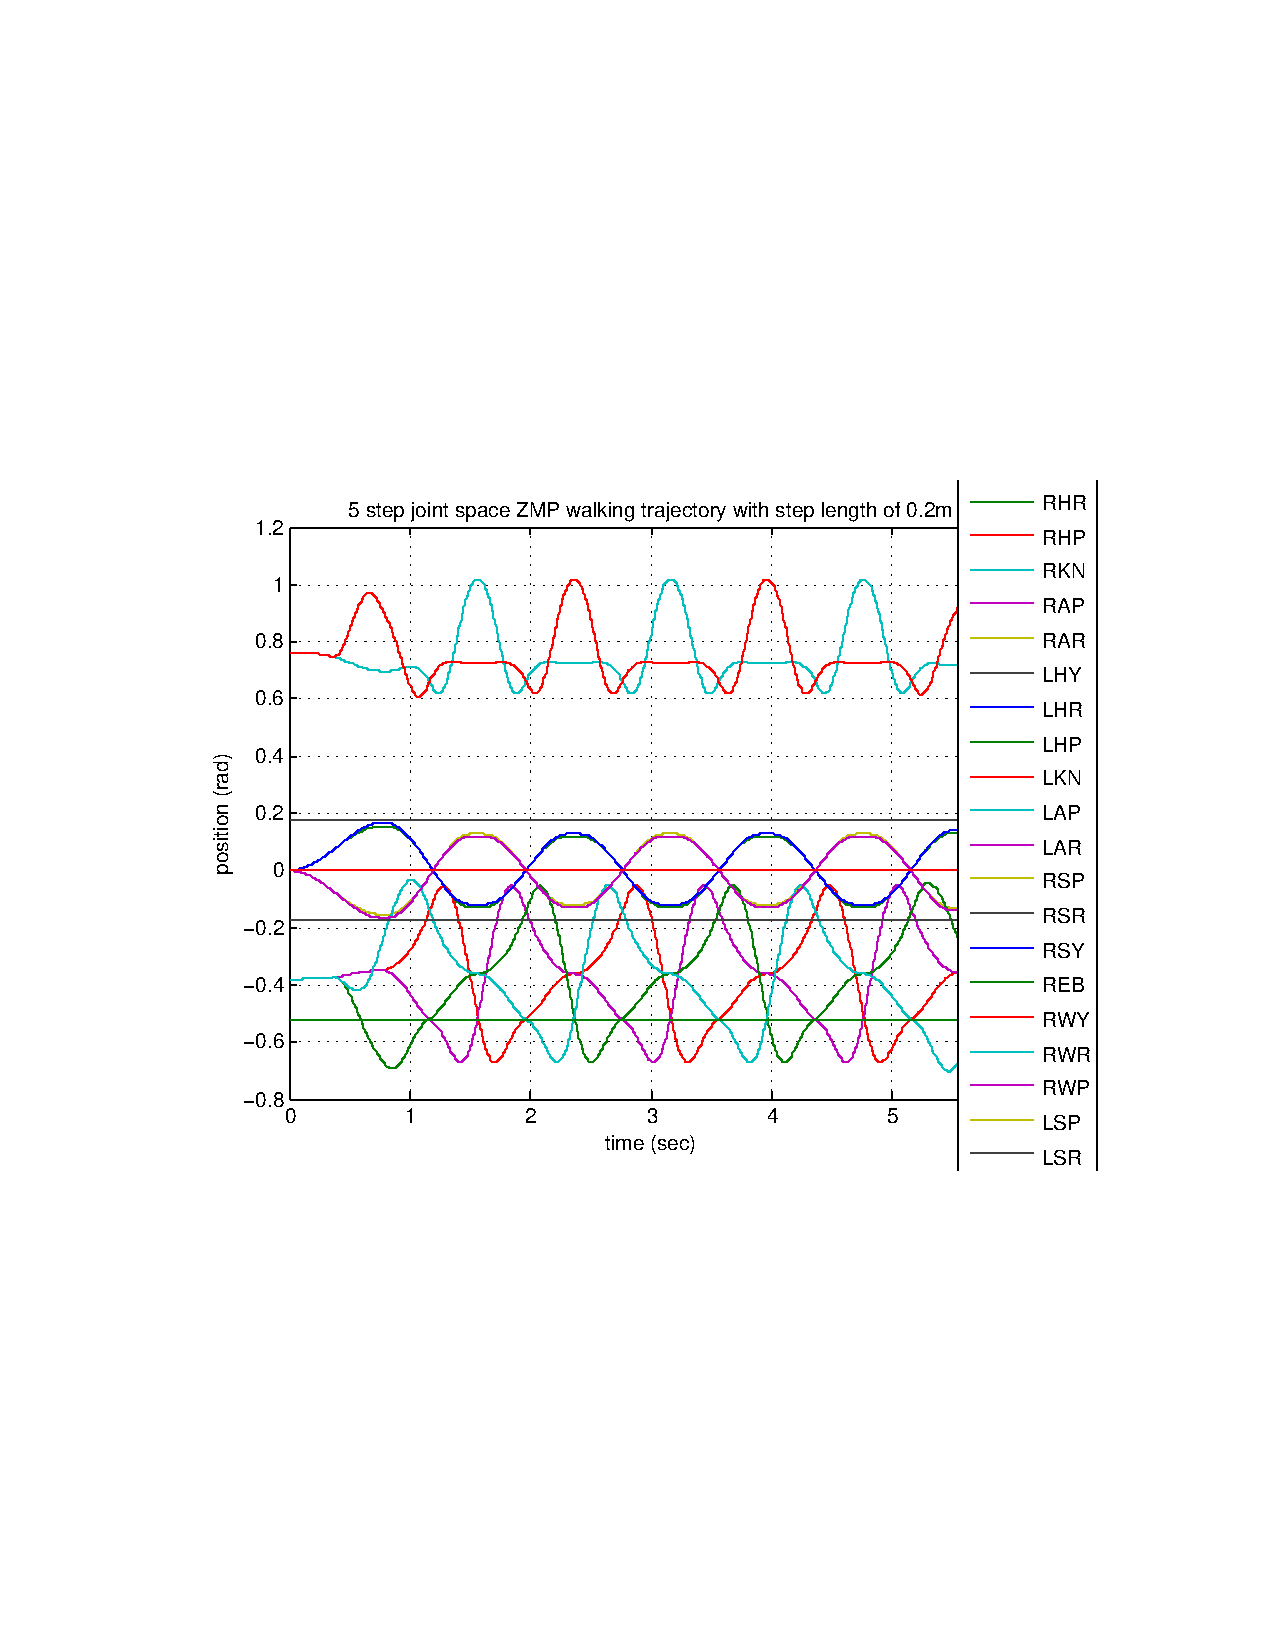
\includegraphics[width=0.8\columnwidth]{./pix/walk5step.pdf}
  \caption{Joint space walking pattern.  The trajectory sampling period $T$ is $0.005~sec$.  Forward step length is $0.2~m$, sway velocity $\widetilde{y}$ is $0.062~\frac{m}{sec}$, and step period is $0.8~sec$.}
  \label{fig:huboZMPjointSpace}
\end{figure}





%% ---------------- OpenHubo Walking ------------------------
\subsection{Walking Using OpenHubo Simulator and Hubo-Ach}\label{sec:OpenHuboWalking}

The walking pattern that was generated in Section~\ref{sec:WalkingPatternGeneration} was then applied to the OpenHubo system described in Section~\ref{sec:simulator} via the Hubo-Ach controller.
The walking pattern was applied in sim-time with a period $T_{sim}$ of $0.005~sec$.
The block diagram of the system using OpenHubo in sim-time for a walking trajectory is shown in Fig.~\ref{fig:openhubosimWalking}.

\begin{figure}
\centering

\begin{tikzpicture}[->,>=stealth',shorten >=1pt,auto,node distance=5cm,
  thick,main node/.style={fill=white!20,draw,font=\sffamily\Large\bfseries}]


  \node[main node] (ctrl) [text width=3cm] {Walking Pattern};
 
  \node[main node] (hubo-ach) [right=1.5cm of ctrl] {Hubo-Ach};
  
  \node[main node,font=\small] (hold1) [right=1.5cm of hubo-ach, yshift=0.5cm] {hold};
  \node[main node,font=\small] (hold2) [right=1.5cm of hubo-ach, yshift=-0.5cm] {hold};
  \node[main node,font=\small] (hold3) [below=0cm of ctrl, yshift=0.0cm] {hold};


  \node[main node] (hubo) [right=1.5cm of hold1, yshift=-0.5cm] {OpenHubo};




%  \path[->, every node/.style={font=\sffamily\small}]
%    (hubo-ach) edge node [above] {$\theta_c$} (hubo);

\draw[->] ([yshift=0.2 cm]hubo-ach.east)  to [out=0,in=-180] node [below] {$\theta_c$} ([yshift=-0.0 cm]hold1.west)  ;
\draw[->] ([yshift=0.0 cm]hold1.east)  to [out=0,in=-180] node [below] {$\theta_c$} ([yshift=0.2 cm]hubo.west)  ;
\draw[-*] ([xshift=1.0 cm]hubo-ach.north)  to [out=60,in=120] node [above] {$\Gamma_{ts}$} ([yshift=-0.05 cm]hold1.north)  ;
%\draw[-*] ([xshift=-0.02 cm]hubo-ach.north)  to [out=120,in=60] node [above] {$\Gamma_{ts}$} ([yshift=-0.05 cm]hold3.north)  ;



\draw[->] ([yshift=0.0 cm]hold2.west)  to [out=180,in=0] node [below] {$H_{state}$} ([yshift=-0.2 cm]hubo-ach.east)  ;
\draw[->] ([yshift=-0.2 cm]hubo.west)  to [out=180,in=0] node [below right] {$H_{state}$} ([yshift=0.0 cm]hold2.east)  ;
\draw[-*] ([xshift=-0.02 cm]hubo.south)  to [out=-120,in=-60] node [above] {$\Gamma_{fs}$} ([yshift=0.05 cm]hold2.south)  ;
\draw[-*] ([xshift=0.02 cm]hubo.south)  to [out=-115,in=-55] node [above] {$\Gamma_{fs}$} ([yshift=0.05 cm]hold3.south)  ;

\draw[-*] (hold3.north)  to [out=90,in=-90] node [above] {}(ctrl.south)  ;

%\draw[->] ([yshift=-0.0 cm]hubo-ach.west)  to [out=180,in=-90] node [below left] {$H_{state}$} ([yshift=0.0 cm]ctrl.south)  ;



%\draw[->] ([yshift=-0.2 cm]hubo.west)  -- node [below] {$H_{state}$} ([yshift=-0.2 cm]hubo-ach.east)  ;
%\draw[->] ([yshift=-0.0 cm]hubo.south)  to [out=-120,in=-60] node [below] {$\Gamma_{fs}$} ([yshift=-0.0 cm]hubo-ach.south)  ;



  \path[->,every node/.style={font=\sffamily\small}]
    (ctrl) edge node [above] {$\theta_r$} (hubo-ach);



\end{tikzpicture}
\caption{Diagram of how the OpenHubo simulator is connected to Hubo-Ach and is used to run a walking trajectory.  
The walking pattern generator ensures proper constraints on the velocity, acceleration and jerk and thus the filter seen in Fig.~\ref{fig:openhubosim} is not desired.  
$\theta_r$ is set directly on the \textbf{FeedForward} channel thus each joint will have the response as seen in Fig.~\ref{fig:singleJointStep} for each commanded reference command at each time step.
Hubo-Ach reads the \textbf{FeedForward} channel and commands Hubo at the rising edge of the next cycle.  
At this point $\Gamma_{ts}$ is set high and the OpenHubo simulator reads $\theta_c$.  
The reference is set within OpenHubo and solved with a simulation period of $T_{sim}$.  
Once The state, $H_{state}$ has been determined it is placed on the Hubo-Ach \textbf{FeedForward} channel and the ready trigger $\Gamma_{fs}$ is raised.  
Hubo-Ach is waiting for the rising edge of $\Gamma_{fs}$ to continue on to the next cycle.  
In order to keep with the sim-time the \textit{Walking Pattern} also waits for the rising edge of $\Gamma_{fs}$ to put the next desired reference on the \textbf{FeedForward} channel. }
\label{fig:openhubosimWalking}
\end{figure}



In Fig.~\ref{fig:openhubosimWalking} the OpenHubo simulator is connected to Hubo-Ach and is used to run the walking trajectory.  
The walking pattern generator ensures proper constraints on the velocity, acceleration and jerk and thus the filter seen in Fig.~\ref{fig:openhubosim} is not desired.  
$\theta_r$ is set directly on the \textbf{FeedForward} channel thus each joint will have the response as seen in Fig.~\ref{fig:singleJointStep} for each commanded reference command at each time step.
Hubo-Ach reads the \textbf{FeedForward} channel and commands Hubo at the rising edge of the next cycle.  
At this point $\Gamma_{ts}$ is set high and the OpenHubo simulator reads $\theta_c$.  
The reference is set within OpenHubo and solved with a simulation period of $T_{sim}$.  
Once The state, $H_{state}$ has been determined it is placed on the Hubo-Ach \textbf{FeedForward} channel and the ready trigger $\Gamma_{fs}$ is raised.  
Hubo-Ach is waiting for the rising edge of $\Gamma_{fs}$ to continue on to the next cycle.  
In order to keep with the sim-time the \textit{Walking Pattern} also waits for the rising edge of $\Gamma_{fs}$ to put the next desired reference on the \textbf{FeedForward} channel.
Fig.~\ref{fig:openHuboWalkingVideo} shows the Virtual Hubo successfully ZMP walking using OpenHubo and Hubo-Ach.

\begin{figure}[thpb]
  \centering
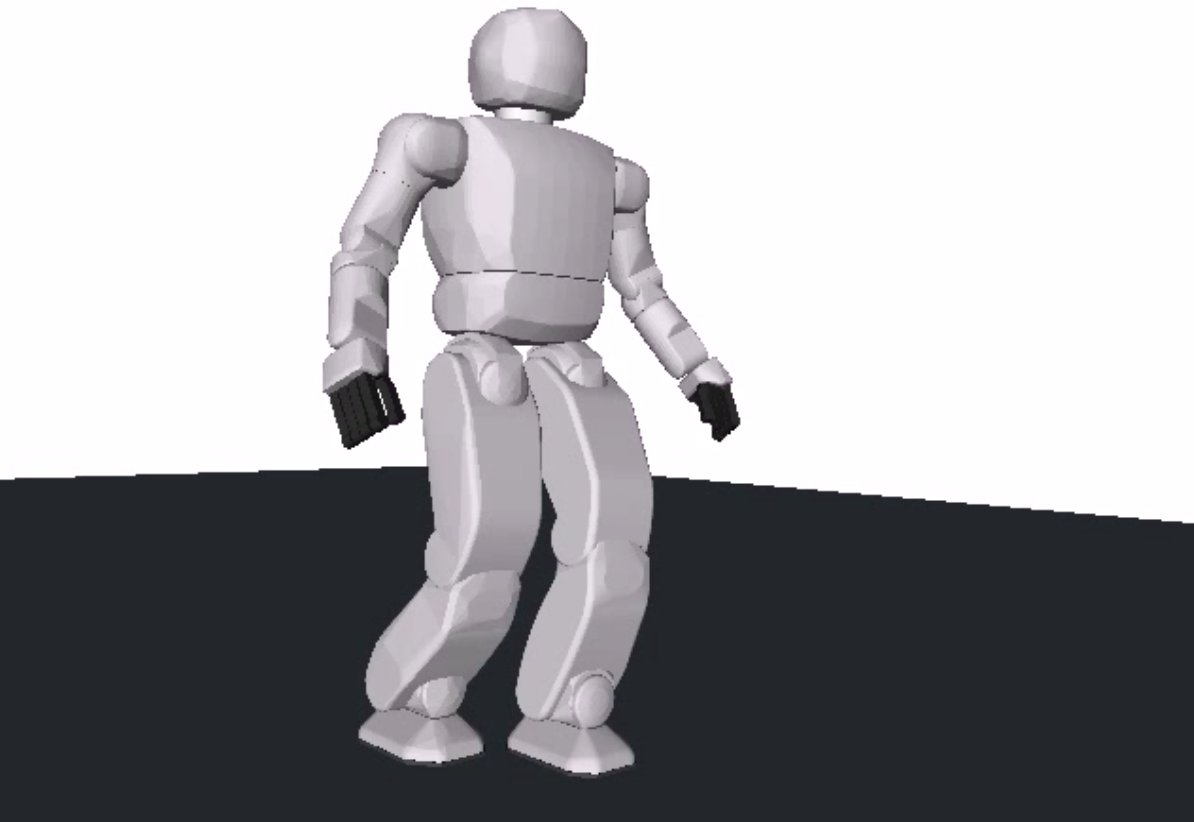
\includegraphics[width=0.6\columnwidth]{./examples/pix/openhubo-walking.png}

\includegraphics[width=0.3\columnwidth]{./qrcode/qrcode-openhubo-walking.png}\\
      Video: http://danlofaro.com/phd/walking/\#WalkingOpenHubo
  \caption{Virtual Hubo in OpenHubo preforming ZMP walking using Hubo-Ach in sim-time based on the walking pattern generated in Section~\ref{sec:WalkingPatternGeneration}}
  \label{fig:openHuboWalkingVideo}
\end{figure}




%% ---------------- OpenHubo Walking ------------------------
\subsection{Walking Using RobotSim and Hubo-Ach}\label{sec:RobotSimWalking}
\begin{figure}[thpb]
  \centering
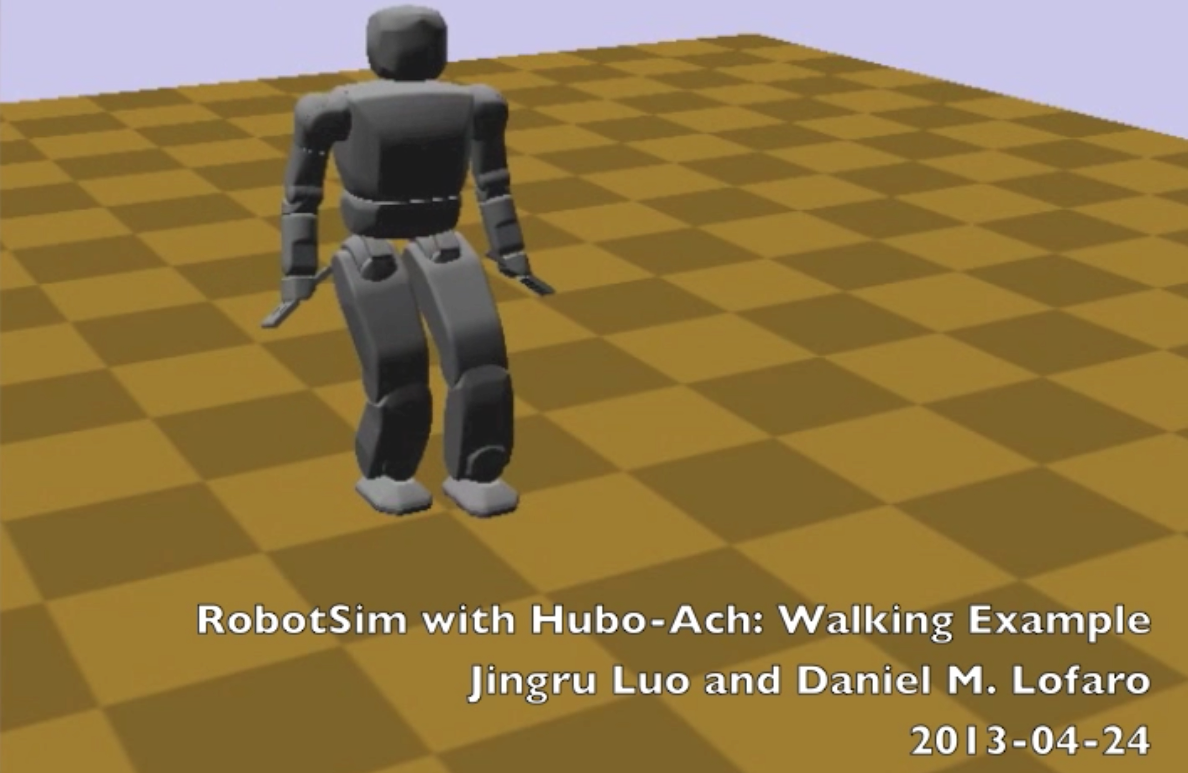
\includegraphics[width=0.6\columnwidth]{./examples/pix/robotsim-walking.png}

\includegraphics[width=0.3\columnwidth]{./qrcode/qrcode-robotsim-walking.png}\\
      Video: http://danlofaro.com/phd/walking/\#WalkingRobotSim
  \caption{Virtual Hubo in RobotSim preforming ZMP walking using Hubo-Ach in sim-time based on the walking pattern generated in Section~\ref{sec:WalkingPatternGeneration}}
  \label{fig:robotSimWalkingVideo}
\end{figure}

The walking pattern that was generated in Section~\ref{sec:WalkingPatternGeneration} was then applied to the RobotSim dynamic simulator via the Hubo-Ach controller.
RobotSim was developed by Professor Kris Hauser from Indiana University.
The simulator was integrated into Hubo-Ach on April 24$^{th}$, 2013 during a 12 hour \textit{Hack-A-Thon} at Worchester Polytechnic Institute by Daniel M. Lofaro, Jingru Luo and Professor Kris Hauser\cite{wpiHackathon}.
The walking pattern was applied in sim-time with a period $T_{sim}$ of $0.005~sec$.
The block diagram of the system using RobotSim in sim-time for a walking trajectory is shown in Fig.~\ref{fig:RobotSimWalking}.

\begin{figure}
\centering

\begin{tikzpicture}[->,>=stealth',shorten >=1pt,auto,node distance=5cm,
  thick,main node/.style={fill=white!20,draw,font=\sffamily\Large\bfseries}]


  \node[main node] (ctrl) [text width=3cm] {Walking Pattern};
 
  \node[main node] (hubo-ach) [right=1.5cm of ctrl] {Hubo-Ach};
  
  \node[main node,font=\small] (hold1) [right=1.5cm of hubo-ach, yshift=0.5cm] {hold};
  \node[main node,font=\small] (hold2) [right=1.5cm of hubo-ach, yshift=-0.5cm] {hold};
  \node[main node,font=\small] (hold3) [below=0cm of ctrl, yshift=0.0cm] {hold};


  \node[main node] (hubo) [right=1.5cm of hold1, yshift=-0.5cm] {OpenHubo};




%  \path[->, every node/.style={font=\sffamily\small}]
%    (hubo-ach) edge node [above] {$\theta_c$} (hubo);

\draw[->] ([yshift=0.2 cm]hubo-ach.east)  to [out=0,in=-180] node [below] {$\theta_c$} ([yshift=-0.0 cm]hold1.west)  ;
\draw[->] ([yshift=0.0 cm]hold1.east)  to [out=0,in=-180] node [below] {$\theta_c$} ([yshift=0.2 cm]hubo.west)  ;
\draw[-*] ([xshift=1.0 cm]hubo-ach.north)  to [out=60,in=120] node [above] {$\Gamma_{ts}$} ([yshift=-0.05 cm]hold1.north)  ;
%\draw[-*] ([xshift=-0.02 cm]hubo-ach.north)  to [out=120,in=60] node [above] {$\Gamma_{ts}$} ([yshift=-0.05 cm]hold3.north)  ;



\draw[->] ([yshift=0.0 cm]hold2.west)  to [out=180,in=0] node [below] {$H_{state}$} ([yshift=-0.2 cm]hubo-ach.east)  ;
\draw[->] ([yshift=-0.2 cm]hubo.west)  to [out=180,in=0] node [below right] {$H_{state}$} ([yshift=0.0 cm]hold2.east)  ;
\draw[-*] ([xshift=-0.02 cm]hubo.south)  to [out=-120,in=-60] node [above] {$\Gamma_{fs}$} ([yshift=0.05 cm]hold2.south)  ;
\draw[-*] ([xshift=0.02 cm]hubo.south)  to [out=-115,in=-55] node [above] {$\Gamma_{fs}$} ([yshift=0.05 cm]hold3.south)  ;

\draw[-*] (hold3.north)  to [out=90,in=-90] node [above] {}(ctrl.south)  ;

%\draw[->] ([yshift=-0.0 cm]hubo-ach.west)  to [out=180,in=-90] node [below left] {$H_{state}$} ([yshift=0.0 cm]ctrl.south)  ;



%\draw[->] ([yshift=-0.2 cm]hubo.west)  -- node [below] {$H_{state}$} ([yshift=-0.2 cm]hubo-ach.east)  ;
%\draw[->] ([yshift=-0.0 cm]hubo.south)  to [out=-120,in=-60] node [below] {$\Gamma_{fs}$} ([yshift=-0.0 cm]hubo-ach.south)  ;



  \path[->,every node/.style={font=\sffamily\small}]
    (ctrl) edge node [above] {$\theta_r$} (hubo-ach);



\end{tikzpicture}
\caption{Diagram of how the OpenHubo simulator is connected to Hubo-Ach and is used to run a walking trajectory.  
The walking pattern generator ensures proper constraints on the velocity, acceleration and jerk and thus the filter seen in Fig.~\ref{fig:openhubosim} is not desired.  
$\theta_r$ is set directly on the \textbf{FeedForward} channel thus each joint will have the response as seen in Fig.~\ref{fig:singleJointStep} for each commanded reference command at each time step.
Hubo-Ach reads the \textbf{FeedForward} channel and commands Hubo at the rising edge of the next cycle.  
At this point $\Gamma_{ts}$ is set high and the OpenHubo simulator reads $\theta_c$.  
The reference is set within OpenHubo and solved with a simulation period of $T_{sim}$.  
Once The state, $H_{state}$ has been determined it is placed on the Hubo-Ach \textbf{FeedForward} channel and the ready trigger $\Gamma_{fs}$ is raised.  
Hubo-Ach is waiting for the rising edge of $\Gamma_{fs}$ to continue on to the next cycle.  
In order to keep with the sim-time the \textit{Walking Pattern} also waits for the rising edge of $\Gamma_{fs}$ to put the next desired reference on the \textbf{FeedForward} channel. }
\label{fig:openhubosimWalking}
\end{figure}



In Fig.~\ref{fig:RobotSimWalking} the RobotSim simulator is connected to Hubo-Ach and is used to run the walking trajectory.  
The walking pattern generator ensures proper constraints on the velocity, acceleration and jerk and thus the filter seen in Fig.~\ref{fig:openhubosim} is not desired.  
$\theta_r$ is set directly on the \textbf{FeedForward} channel thus each joint will have the response as seen in Fig.~\ref{fig:singleJointStep} for each commanded reference command at each time step.
Hubo-Ach reads the \textbf{FeedForward} channel and commands Hubo at the rising edge of the next cycle.  
At this point $\Gamma_{ts}$ is set high and the RobotSim simulator reads $\theta_c$.  
The reference is set within RobotSim and solved with a simulation period of $T_{sim}$.  
Once The state, $H_{state}$ has been determined it is placed on the Hubo-Ach \textbf{FeedForward} channel and the ready trigger $\Gamma_{fs}$ is raised.  
Hubo-Ach is waiting for the rising edge of $\Gamma_{fs}$ to continue on to the next cycle.  
In order to keep with the sim-time the \textit{Walking Pattern} also waits for the rising edge of $\Gamma_{fs}$ to put the next desired reference on the \textbf{FeedForward} channel.
Fig.~\ref{fig:robotSimWalkingVideo} shows the Virtual Hubo successfully ZMP walking using RobotSim and Hubo-Ach.

\begin{figure}
\centering

\begin{tikzpicture}[->,>=stealth',shorten >=1pt,auto,node distance=5cm,
  thick,main node/.style={fill=white!20,draw,font=\sffamily\Large\bfseries}]


  \node[main node] (ctrl) [text width=3cm] {Walking Pattern};
 
  \node[main node] (hubo-ach) [right=1.5cm of ctrl] {Hubo-Ach};
  
  \node[main node,font=\small] (hold1) [right=1.5cm of hubo-ach, yshift=0.5cm] {hold};
  \node[main node,font=\small] (hold2) [right=1.5cm of hubo-ach, yshift=-0.5cm] {hold};
  \node[main node,font=\small] (hold3) [below=0.0cm of ctrl, yshift=0.0cm] {hold};


  \node[main node] (hubo) [right=1.5cm of hold1, yshift=-0.5cm] {RobotSim};




%  \path[->, every node/.style={font=\sffamily\small}]
%    (hubo-ach) edge node [above] {$\theta_c$} (hubo);

\draw[->] ([yshift=0.2 cm]hubo-ach.east)  to [out=0,in=-180] node [below] {$\theta_c$} ([yshift=-0.0 cm]hold1.west)  ;
\draw[->] ([yshift=0.0 cm]hold1.east)  to [out=0,in=-180] node [below] {$\theta_c$} ([yshift=0.2 cm]hubo.west)  ;
\draw[-*] ([xshift=1.0 cm]hubo-ach.north)  to [out=60,in=120] node [above] {$\Gamma_{ts}$} ([yshift=-0.05 cm]hold1.north)  ;
%\draw[-*] ([xshift=-0.02 cm]hubo-ach.north)  to [out=120,in=60] node [above] {$\Gamma_{ts}$} ([yshift=-0.05 cm]hold3.north)  ;



\draw[->] ([yshift=0.0 cm]hold2.west)  to [out=180,in=0] node [below] {$H_{state}$} ([yshift=-0.2 cm]hubo-ach.east)  ;
\draw[->] ([yshift=-0.2 cm]hubo.west)  to [out=180,in=0] node [below right] {$H_{state}$} ([yshift=0.0 cm]hold2.east)  ;
\draw[-*] ([xshift=-0.02 cm]hubo.south)  to [out=-120,in=-60] node [above] {$\Gamma_{fs}$} ([yshift=0.05 cm]hold2.south)  ;
\draw[-*] ([xshift=0.02 cm]hubo.south)  to [out=-115,in=-55] node [above] {$\Gamma_{fs}$} ([yshift=0.05 cm]hold3.south)  ;

\draw[-*] (hold3.north)  to [out=90,in=-90] node [above] {}(ctrl.south)  ;

%\draw[->] ([yshift=-0.0 cm]hubo-ach.west)  to [out=180,in=-90] node [below left] {$H_{state}$} ([yshift=0.0 cm]ctrl.south)  ;



%\draw[->] ([yshift=-0.2 cm]hubo.west)  -- node [below] {$H_{state}$} ([yshift=-0.2 cm]hubo-ach.east)  ;
%\draw[->] ([yshift=-0.0 cm]hubo.south)  to [out=-120,in=-60] node [below] {$\Gamma_{fs}$} ([yshift=-0.0 cm]hubo-ach.south)  ;



  \path[->,every node/.style={font=\sffamily\small}]
    (ctrl) edge node [above] {$\theta_r$} (hubo-ach);



\end{tikzpicture}
\caption{Diagram of how the RobotSim simulator is connected to Hubo-Ach and is used to run the walking trajectory.  
The walking pattern generator ensures proper constraints on the velocity, acceleration and jerk and thus the filter seen in Fig.~\ref{fig:openhubosim} is not desired.  
$\theta_r$ is set directly on the \textbf{FeedForward} channel thus each joint will have the response as seen in Fig.~\ref{fig:singleJointStep} for each commanded reference command at each time step.
Hubo-Ach reads the \textbf{FeedForward} channel and commands Hubo at the rising edge of the next cycle.  
At this point $\Gamma_{ts}$ is set high and the RobotSim simulator reads $\theta_c$.  
The reference is set within RobotSim and solved with a simulation period of $T_{sim}$.  
Once The state, $H_{state}$ has been determined it is placed on the Hubo-Ach \textbf{FeedForward} channel and the ready trigger $\Gamma_{fs}$ is raised.  
Hubo-Ach is waiting for the rising edge of $\Gamma_{fs}$ to continue on to the next cycle.  
In order to keep with the sim-time the \textit{Walking Pattern} also waits for the rising edge of $\Gamma_{fs}$ to put the next desired reference on the \textbf{FeedForward} channel.}
\label{fig:RobotSimWalking}
\end{figure}







%% ---------------- Hubo Walking ------------------------
\subsection{Hubo Walking using Hubo-Ach}\label{sec:HuboWalking}
The walking pattern that was generated in Section~\ref{sec:WalkingPatternGeneration} was then applied to the physical Hubo platform using the Hubo-Ach controller.
The walking pattern was applied in real-time with a period $T_r$ of $0.005~sec$.
Unlike the simulated versions which run in sim-time the system is now running in real-time; thus it no longer needs to wait for an external trigger.
The walking pattern trajectory is now posted to the \textbf{FeedForward} channel at an RT period of $T_r$.
The walking pattern generator ensures proper constraints on the velocity, acceleration and jerk and thus the filter seen in Fig.~\ref{fig:openhubosim} is not desired.
Fig.~\ref{fig:huboWalk} shows the block diagram of the walking pattern from Section~\ref{sec:WalkingPatternGeneration} being run in real-time on the physical Hubo2+ platform.
Fig.~\ref{fig:RealHuboWalkingVideo} shows the Hubo successfully ZMP walking using OpenHubo and Hubo-Ach.
Fig.~\ref{fig:RealHuboWalkingInPlaceVideo} shows the Hubo successfully ZMP walking in place using OpenHubo and Hubo-Ach.


\begin{figure}
\centering
\begin{tikzpicture}[->,>=stealth',shorten >=1pt,auto,node distance=5cm,
  thick,main node/.style={fill=white!20,draw,font=\sffamily\Large\bfseries}]


  \node[main node] (ref) {Walking Pattern};
  \node[main node] (hubo-ach) [right=2.5cm of ref] {Hubo-Ach};
  \node[main node] (hubo) [right=2.5cm of hubo-ach] {Hubo};




  \path[<->,dashed, every node/.style={font=\sffamily\small}]
    (hubo) edge node [above] {CAN} (hubo-ach);

  \path[->,every node/.style={font=\sffamily\small}]
    (ref) edge node [above] {$\theta_r$} (hubo-ach);


\end{tikzpicture}
\caption{Reference $\theta_r$ being applied to Hubo via Hubo-Ach.  $\theta_r$ is set on the \textbf{FeedForward} channel, Hubo-Ach reads it then commands Hubo at the rising edge of the next cycle.}
\label{fig:huboWalk}
\end{figure}




\begin{figure}[thpb]
  \centering
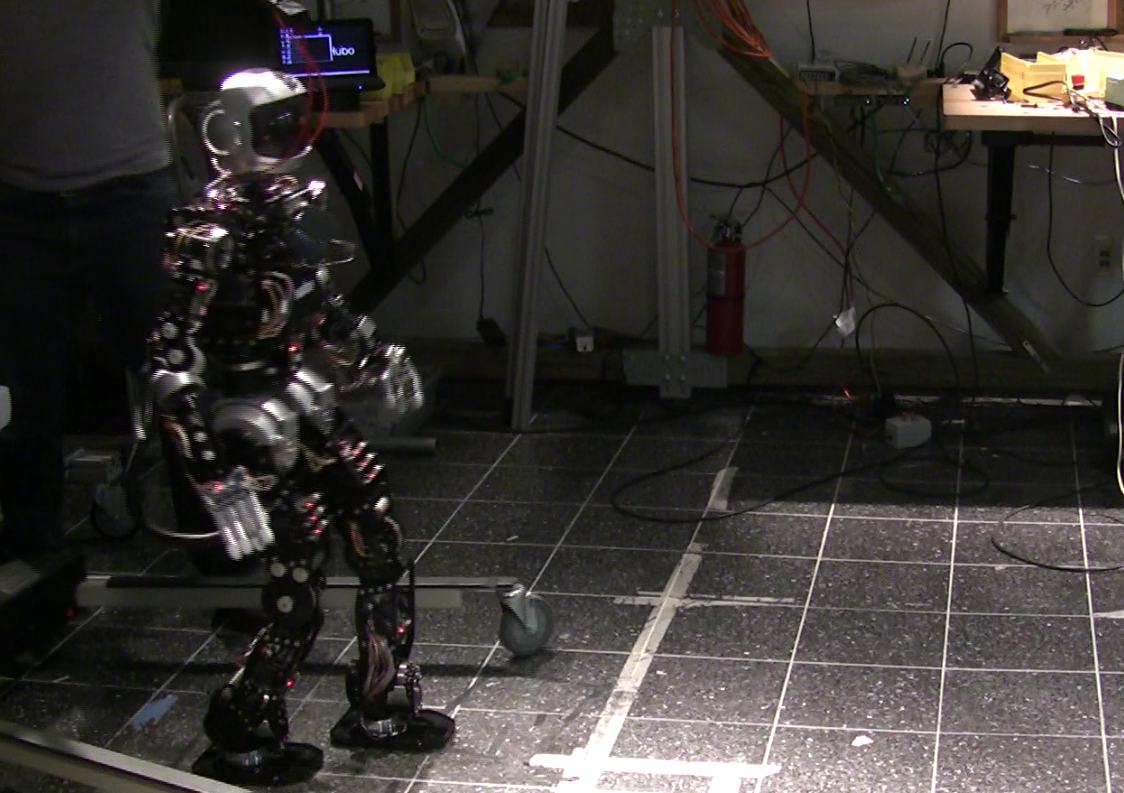
\includegraphics[width=0.6\columnwidth]{./examples/pix/hubo-walking.png}

\includegraphics[width=0.3\columnwidth]{./qrcode/qrcode-hubo-walking.png}\\
      Video: http://danlofaro.com/phd/walking/\#WalkingHubo
  \caption{Hubo2+ preforming ZMP walking using Hubo-Ach in real-time based on the walking pattern generated in Section~\ref{sec:WalkingPatternGeneration}.}
  \label{fig:RealHuboWalkingVideo}
\end{figure}

\begin{figure}[thpb]
  \centering
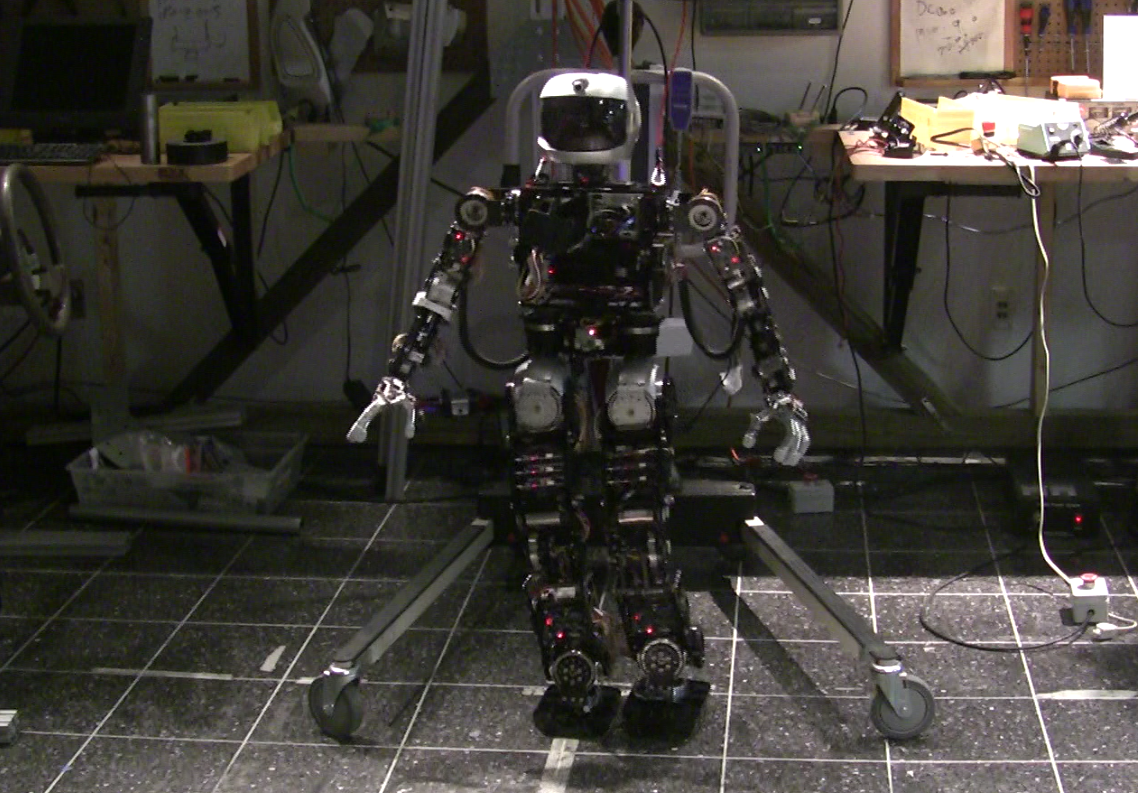
\includegraphics[width=0.6\columnwidth]{./examples/pix/hubo-walkinginplace.png}

\includegraphics[width=0.3\columnwidth]{./qrcode/qrcode-hubo-walkinginplace.png}\\
      Video: http://danlofaro.com/phd/walking/\#WalkingInPlaceHubo
  \caption{Hubo2+ preforming ZMP walking in place using Hubo-Ach in real-time based on the walking pattern generated in Section~\ref{sec:WalkingPatternGeneration} with a forward velocity of $0.0~\frac{m}{sec}$}
  \label{fig:RealHuboWalkingInPlaceVideo}
\end{figure}





%% ---------------- Hubo Walking in 5 days ------------------------
\subsection{Hubo Dynamic Walking - Developed in 5 Days Using Hubo-Ach}\label{sec:dynamicWalking}
Fig.~\ref{fig:dynamicwalking} shows Hubo2+ dynamic walking using Hubo-Ach as the primary controller.  The standard ZMP walking algorithms were implemented by our partners Mike Sillman and Matt Zucker at Geortia Gech and Swarthmore respectively.  All control was implemented using Daniel M. Lofaro's Hubo-Ach system.

\begin{figure}[thpb]
  \centering
  %\begin{tikzpicture}
    %\clip [rounded corners=1em] (0,0) rectangle coordinate (centerpoint) (5,7.5cm);
%    \node[minimum width=\linewidth,minimum height=174pt,draw=black,rounded corners=1em,fill=bgcolor,draw=black]
%    {};
%    \node[name=img] {
      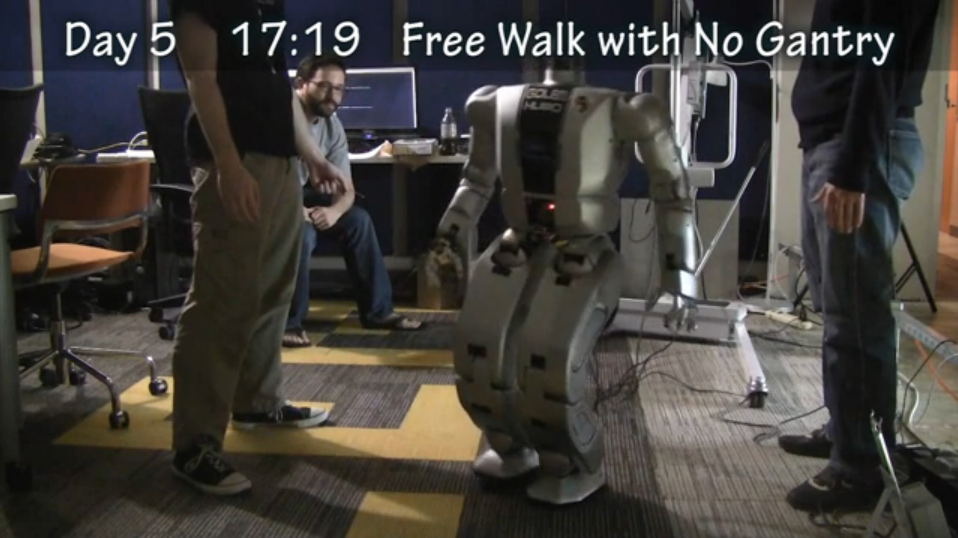
\includegraphics[width=0.6\columnwidth]{./examples/pix/dynamicwalking.png}
      
\includegraphics[width=0.3\columnwidth]{./qrcode/qrcode-dynamicwalking.png}\\
      Video: http://danlofaro.com/phd/walking/\#Walking5Days
%    };
%    \draw [bgcolor, rounded corners=1em, line width=1em,inner sep=0pt]
%    (img.north west) --
%    (img.north east) --
%    (img.south east) --
%    (img.south west) -- cycle
%    ;
%  \end{tikzpicture}
\caption{Hubo dynamic walking using Hubo-Ach as the primary controller.  The standard ZMP walking algorithms were implemented by our partners Mike Sillman and Matt Zucker at Geortia Gech and Swarthmore respectively.  All control was implemented using Daniel M. Lofaro's Hubo-Ach system.}
  \label{fig:dynamicwalking}
\end{figure}











	\subsection{Static Walking}\label{sec:staticWalking}
		\begin{figure}[thpb]
  \centering
  %\begin{tikzpicture}
    %\clip [rounded corners=1em] (0,0) rectangle coordinate (centerpoint) (5,7.5cm);
%    \node[minimum width=\linewidth,minimum height=174pt,draw=black,rounded corners=1em,fill=bgcolor,draw=black]
%    {};
%    \node[name=img] {
      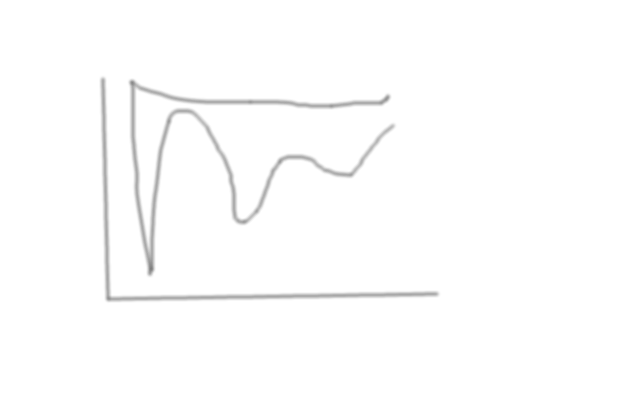
\includegraphics[width=0.93\columnwidth]{./pix/tmp.png}
      
\includegraphics{./qrcode/qrcode-staticwalking.png}\\
      Video: http://danlofaro.com/phd/staticwalking/
%    };
%    \draw [bgcolor, rounded corners=1em, line width=1em,inner sep=0pt]
%    (img.north west) --
%    (img.north east) --
%    (img.south east) --
%    (img.south west) -- cycle
%    ;
%  \end{tikzpicture}
\caption{Hubo static walking using Hubo-Ach as the primary controller.  The static walking algorithm was implimented by Youngbum Jun.  All control was
implimented using Daniel M. Lofaro's Hubo-Ach system.
}
  \label{fig:staticwalking}
\end{figure}

	\subsection{Dynamic Walking}\label{sec:dynamicWalking}
		\begin{figure}[thpb]
  \centering
  %\begin{tikzpicture}
    %\clip [rounded corners=1em] (0,0) rectangle coordinate (centerpoint) (5,7.5cm);
%    \node[minimum width=\linewidth,minimum height=174pt,draw=black,rounded corners=1em,fill=bgcolor,draw=black]
%    {};
%    \node[name=img] {
      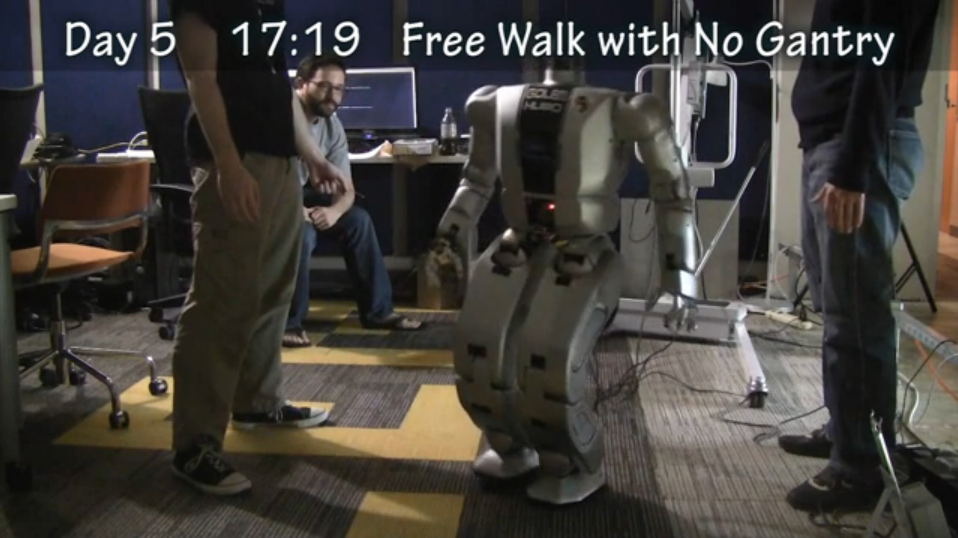
\includegraphics[width=0.93\columnwidth]{./examples/pix/dynamicwalking.png}
      
\includegraphics{./qrcode/qrcode-dynamicwalking.png}\\
      Video: http://danlofaro.com/phd/dynamicwalking/
%    };
%    \draw [bgcolor, rounded corners=1em, line width=1em,inner sep=0pt]
%    (img.north west) --
%    (img.north east) --
%    (img.south east) --
%    (img.south west) -- cycle
%    ;
%  \end{tikzpicture}
\caption{Hubo dynamic walking using Hubo-Ach as the primary controller.  The standard dynamic walking algorithms were implimented by our partners Mike Sillman and Matt Zucker at Geortia Gech and Swarthmore respectively.  All control was implimented using Daniel M. Lofaro's Hubo-Ach system.}
  \label{fig:dynamicwalking}
\end{figure}















\section{Simulator}\label{sec:simulator}
Hubo-Ach is designed to run in either real-time or in simulation time.
This is especially useful when running experimental controllers and you do not want to damage the robot.
In real-time mode Hubo-Ach updates at its normal 


\section{Task}\label{sec:task}
Turning a valve with whole body (more of a lever)
\begin{itemize}
\item Find the valve - sensing
\item Move to the valve - close loop on sensing
\item Grab the valve
\item Jump on the valve
\end{itemize}



\section{System setup}

State diagram of plan
\begin{itemize}
\item Find the valve - sensing
\item Move to the valve - close loop on sensing
\item Grab the valve
\item Jump on the valve
\end{itemize}

Software structrue
\begin{itemize}
\item Hubo-Ach
\item ROS (the connectiving with latency/non-real time problem)

\item Etc.
\end{itemize}


Sensors Chosen
\begin{itemize}
\item FT
\item IMU
\item Monocular
\item RGB-D
\end{itemize}

Controllers
\begin{itemize}
\item Walking
\item Balance
\item Complience
\item IK
\item Visual Servoing
\end{itemize}

\section{Results}\label{sec:results}
\begin{itemize}
\item What worked
\item What did not
\item To be improved
\end{itemize}
